% !TeX root = ../thuthesis-example.tex

\begin{translation}
\label{cha:translation}

\title{张量代数编译转移空间\cite{kjolstad:2019:workspaces}}
\maketitle

\tableofcontents

\section{摘要}

本文展示了如何扩展稀疏张量代数编译器以引入称为转移空间的临时张量,以避免低效的稀疏数据结构访问。我们为张量运算开发了一种称为具体索引符号的中间表示法 (IR),
它指定子计算何时发生以及它们的存储位置。然后,我们将描述此IR中的转移空间转换、如何以编程方式调用它以及如何将 IR 编译为稀疏代码。
最后,我们展示了如何使用该变换来优化稀疏张量算子,包括稀疏矩阵乘法、稀疏张量加法和矩阵化张量乘以Khatri-Rao积(MTTKRP)。我们的结果表明,
转移空间转换使这些算子的性能与手动优化的实现相当。例如,我们将具有密集输出的 MTTKRP 的性能提高了高达 35\%,
并能够生成稀疏矩阵乘法和具有稀疏输出的 MTTKRP。之前的张量代数编译器均不能支持这两种算子。



\section{介绍}

临时标量变量对于优化遍历密集多维数组和表示张量的稀疏压缩数据结构的循环很重要。 变量访问起来很方便,因为它们不需要地址计算,可以存储在寄存器中,
也可以用于预先计算循环不变表达式。 临时变量也可以是我们称之为转移空间的高维张量。 由于更简单的地址计算和更好的局部性,低维度的转移空间(例如向量)比高维度的张量更容易访问。
这使得它们可以加速重复访问张量切片的循环,并且它们还可以用于预计算循环不变的高维张量表达式。
转移空间为优化在稀疏张量上计算的循环提供了额外的机会。 稀疏张量主要包含零,因此存储在压缩的不规则数据结构中。 渐近复杂度下更快的随机访问和插入,
稠密转移空间在替代压缩张量时可以大大降低访问和插入成本。(随机访问压缩张量的时间复杂度为 $O(log n)$ ,这一复杂度来自搜索。插入复杂度为 $O(n)$,这一复杂度来自数据搬移。)
此外,在稀疏张量代码中常见的压缩数据结构的同时迭代需要合并有很多条件的循环。 通过引入低维度的稠密张量转移空间来保持最小的内存成本,
我们可以降低插入成本并用随机访问替换合并循环。

先前关于稀疏张量编译的工作描述了如何优化稀疏命令式代码,以及如何从高级张量索引符号生成稀疏代码。 但是,它们没有考虑引入临时张量的优化。 
这些在许多稀疏张量算子中很重要,例如张量加法、稀疏矩阵乘法(其中所有矩阵都是稀疏的),以及用于分解稀疏张量的矩阵化张量乘以Khatri-Rao积(MTTKRP)。 
如果没有编译器对转移空间的支持,我们就会丢失性能优化的机会。 事实上,稀疏矩阵乘法算子在没有转移空间的情况下会在渐近复杂度意义下变慢。
本文介绍了一种编译器转换,它将临时张量转移空间引入到我们之前的工作TACO中。 从张量索引符号生成的稀疏代码中。 
这种转移空间转换以称为具体索引表示法的新中间表示法(IR)表示,它精确地描述了计算发生的时间和结果的存储位置。 
转移空间转换通过调度API以编程方式调用,让用户控制何时应用它。 我们概述了调用转换的启发式方法,但将确定稀疏张量代数表达式的完整调度空间的策略系统作为未来的工作。 
这个策略系统可以建立在我们的调度API之上。
本文的贡献是:
\begin{itemize}
 \item 具体索引符号(Concrete Index Notation)。 我们引入了一种新的张量代数IR,它指定循环顺序和临时变量。
 \item 转移空间转换(Workspace Transformation)。我们描述了一个张量代数编译器转换,它可以用来移除昂贵的稀疏张量随机插入、消除合并代码和提升循环不变代码。
 \item 编译(Compilation)。我们在之前工作的基础上将具体索引符号编译为稀疏代码。
 \item 案例研究(Case Studies) 我们展示了转换如何从文献中重新创建稀疏矩阵乘法、稀疏矩阵加法和MTTKRP算法,同时推广到新算子。
\end{itemize}
在贡献评估方面,我们展示了使用转移空间带来的性能改进、观察到某些算子获得渐近性能改进。我们展示了生成的稀疏代码的性能与英特尔MKL库、Eigen库和SPLATT高性能库中的手动优化实现相比具有竞争力的性能结果。
最终性能实验显示,稀疏矩阵乘法相较于Eigen加速4倍和MKL加速1.28 倍。


\section{预计算调度指令}
我们基于Halide中计算-调度分离的思想,提出了对TACO的调度扩展,以支持以编程方式重新排序循环并将子表达式预计算到转移空间中。 
重新排序和预计算调度方法调用转移空间转换(Workspace Transformation)和重新排序转换(Reorder Transformation)。以C++语法声明预计算接口如图~\ref{fig:precompute-defination}所示。
\begin{figure}
  \centering
  \subcaptionbox{预计算调度接口\label{fig:precompute-defination}}
    {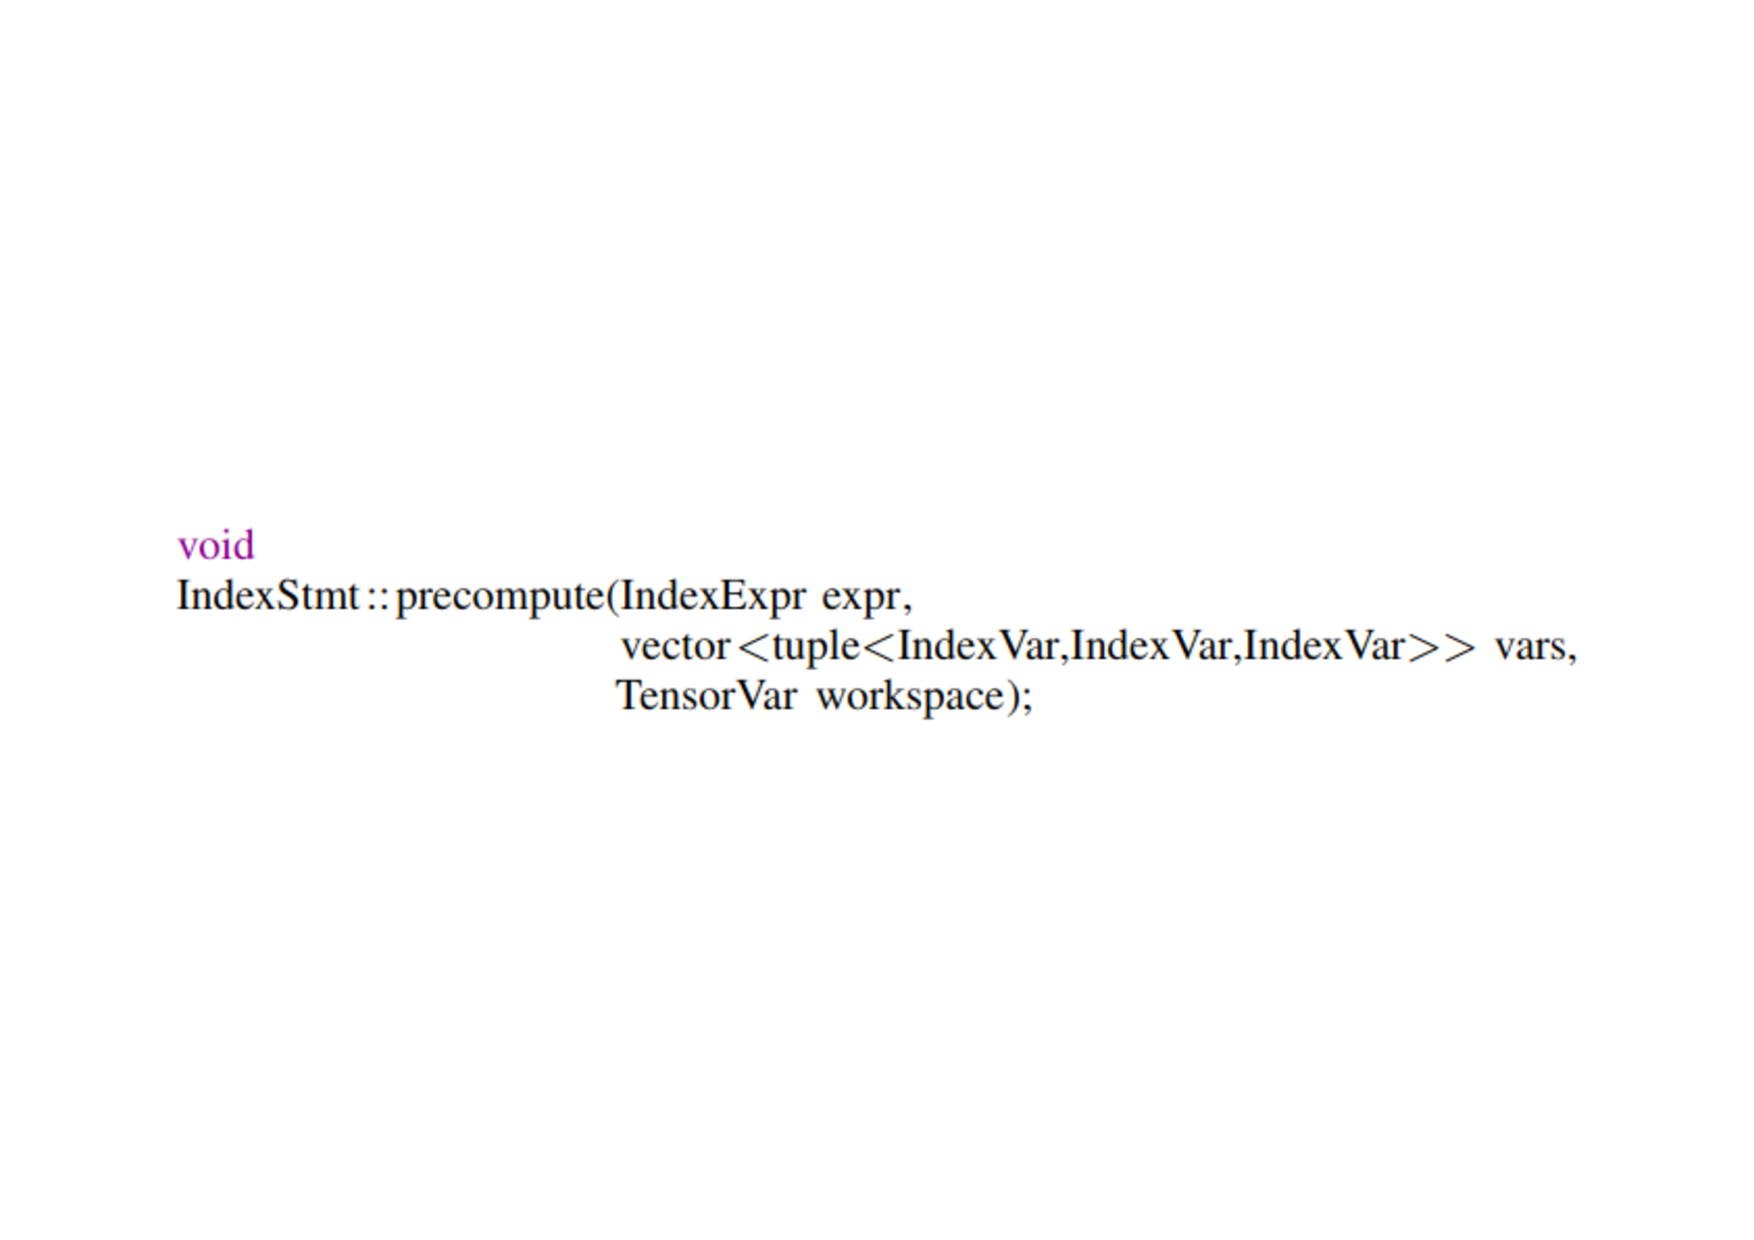
\includegraphics[width=0.35\linewidth]{Precompute-Defination.pdf}}
  \subcaptionbox{预计算调度使用示例\label{fig:c-example}}
    {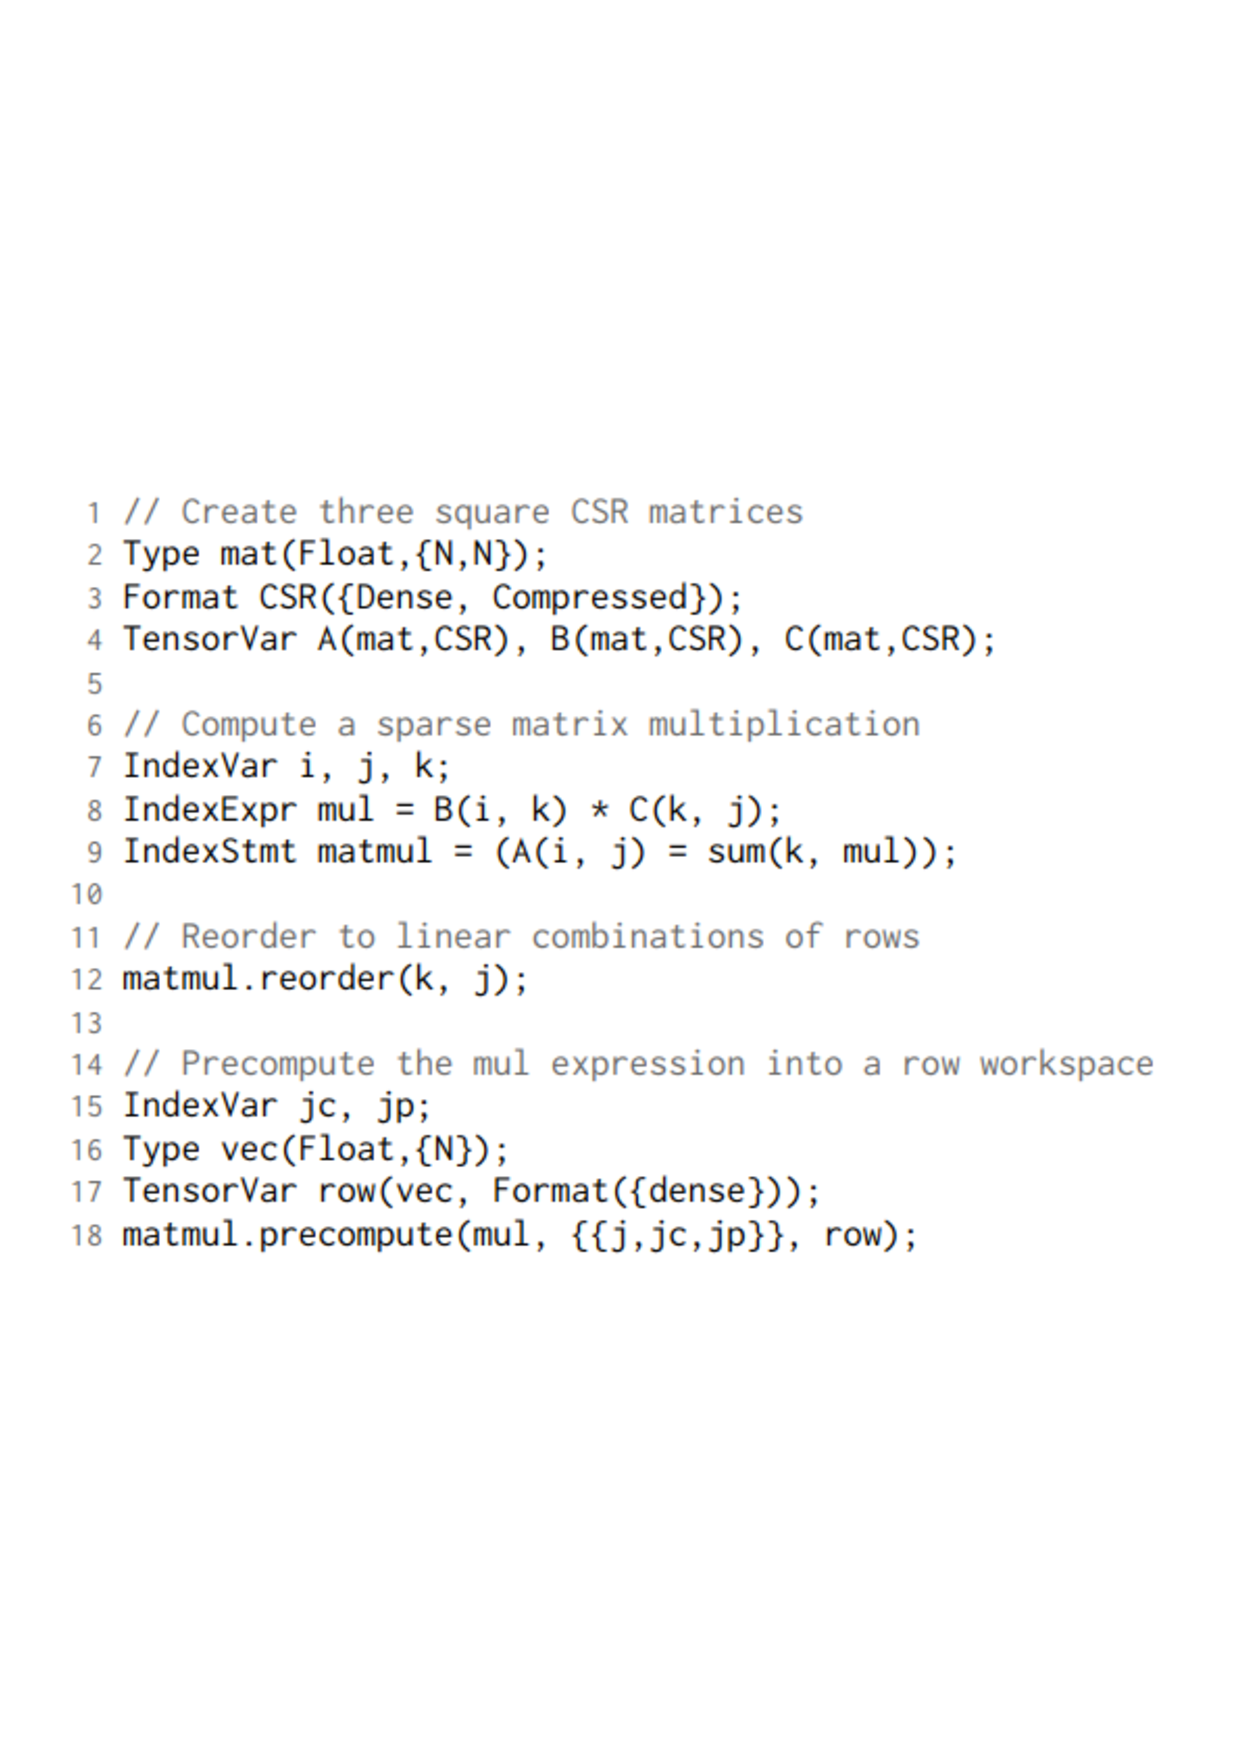
\includegraphics[width=0.35\linewidth]{C++Example.pdf}}
  \caption{预计算调度}
  \label{fig:precomputes}
\end{figure}


我们将预计算方法应用于索引符号语句,并提供要预计算的表达式、要预计算的索引变量以及存储预计算结果的转移空间作为参数。 
expr参数是一个索引表达式,包含在我们调用预计算的索引语句中。vars参数是形式为(old, consumer, producer)的索引变量三元组的向量。 
旧索引变量(old)是我们希望预先计算的变量,它被分成消费者(consumer)和生产者(producer)索引变量。 
生产者变量用于迭代计算转移空间的语句,消费者变量用于迭代使用转移空间的语句。 
最后,转移空间参数是一个张量,用于存储预先计算的结果,其顺序和维度必须足够大以包含所有临时值。
图~\ref{fig:c-example}显示了一个C++示例,它使用重新排序和预计算方法来转换索引表示法语句。
第 2-4 行创建三个具有单精度浮点分量A、B和C的CSR方阵。第7-9行使用索引符号API创建矩阵乘法表达式。
循环的初始顺序是ijk,形成一个内积矩阵乘法算法。 然而,矩阵以CSR行优先矩阵格式存储,因此具有$ C_{kj}$ 访问的ijk循环顺序导致C矩阵在列优先方向上访问。
行优先稀疏矩阵的列优先访问渐近效率低下。 因此,第 12 行对k和j进行重新排序,使对C的访问成为行优先的,并形成行矩阵乘法算法的ikj线性组合。 
然而,重新排序引入了新的效率地下问题。由于 $ A_{ij} $ 中使用的j索引变量现在位于k求和索引变量内,因此代码会将值分散到A中。
但是,A的CSR格式不支持高效随机插入的行优先。因此,第15-18行预先计算并将结果分散到一个稠密的行转移空间中,然后将其复制到A。
稠密转移空间很有用,因为它们支持$ O(1) $随机访问和插入。然而,转移空间可以是任何格式,包括压缩和哈希映射。特别地,哈希映射还支持$ O(1) $随机访问和插入,而无需存储所有零。
此外,转移空间的组件类型可以不同于操作数和结果张量,从而可以使用混合精度算法。例如,图~\ref{fig:c-example}中的行转移空间可以用双精度浮点组件构造,以更高精度地累加值。

\section{具体索引符号}
索引符号是张量代数代码生成器和框架的一种流行输入语言。它描述了张量操作应该做什么,独立于它们的计算方式和访问张量的方式。因此,优化决策不会与算法描述混合。
虽然索引符号是适合张量运算的输入语言,但它不适合作为编译器IR。原因是它没有指定执行顺序或临时张量及其格式。
可以使用几种现有的表示法来完整描述索引表达式的计算方式,例如实现索引表达式的低层次C代码、多面体模型的稀疏扩展或迭代图. 
然而,这些表示自由度过高,无法方便地应用本文中描述的转移空间转换。
我们提出了一种新的张量运算中间语言,称为具体索引符号(Concrete Index Notation)。
具体索引符号使用描述循环顺序、在哪里使用临时变量和临时变量格式的结构来扩展索引符号,但没有关于如何在稀疏数据结构上进行协作的细节。
在编译器软件堆栈中,具体索引表示法是索引表示法和低级命令式IR之间的中间表示。
这种设计的一个好处是我们可以转换具体的索引符号,而不是转换具有间接访问、条件和while循环的稀疏命令式代码。然后在降低具体索引符号时生成稀疏命令式代码。

具体的索引表示法有四种语句类型。赋值(assignment)语句将表达式的结果分配给张量分量,循环(forall)语句在从张量维度推断出的范围内执行语句,暂存(where)语句创建存储子表达式的临时对象,
以及序列(sequence)语句重用临时变量。
为了描述具体的索引符号,我们回到行矩阵乘法示例的线性组合。 我们以ikj顺序用 forall循环表达算法 $\forall_{ikj} A_ij +=B_{ik}C_{kj}$
赋值语句修改单个张量分量的值。它可以是常规赋值(=)或递增赋值(例如,+=,但也允许使用其他运算符)。
在矩阵乘法示例中,递增赋值语句 $ A_{ij} += B_{ik}C_{kj} $ 修改张量分量$ A_{ij} $的值。该语句受到限制,左侧的张量可能不会出现在表达式的右侧,
并且仅使用索引变量访问每个张量。 最后,结果张量被隐式初始化为零。
循环语句通过将索引变量绑定到一组值来表示迭代。循环语句的嵌套描述了索引变量被迭代的顺序。在矩阵乘法示例中,三个forall语句$ \forall_i\forall_k\forall_j $,简写为$\forall_{ikj}$,指定迭代顺序。
暂存语句提前将一个表达式计算结果存储到一个临时的张量变量中。矩阵乘法算法将被方所过的行重复计算和累加到输出矩阵A中。如果A是按照分段压缩格式存储,向行中插入的代价会很高,所以我们可以用一个暂存语句将部分结果累加到一个稠密转移空间中 $\forall_i(\forall_j A_{ij}=w_j) where (\forall_{kj}w_j+=B_{ik}C_{kj})$。
暂存语句引入一个稠密向量$w$来存放右手侧生产者产生的每一行的部分和,然后再复制到左手侧消费者$A$中。
序列语句允许更新张量。假设我们想要把一个CSR格式存储的稀疏矩阵D加到B和C的乘积中。这个操作$ A = D+ BC$ 最好通过服用稠密临时向量$w$实现。与暂存语句不同,一个序列语句中定义在左手侧的张量可以被右手侧张量修改。因此他们可以被用来表达序列的张量写入。


出于多种原因,重新排序具体的索引符号语句很有用。 首先,稀疏张量对它们的访问顺序很敏感。 例如,迭代CSC矩阵的行成本很高,因此我们可以对所有语句重新排序以产生更好的访问模式。
我们可能还希望重新排序以将循环不变的where语句移出内部循环。至关重要的是,我们可能需要重新排序语句,以便我们的转移空间转换的先决条件适用。
当我们重新排序一个具体的索引语句时,我们想知道它会像以前一样做同样的事情。我们可以通过将较大的重新排序操作分解为较小的等价来确保语义等价。
在所有情况下,我们都要求所有被重新排序的语句不包含序列语句。 交换forall语句需要关联属性。如果S是一个用赋值语句修改其张量的语句或用结合运算符的增量语句,
那么 $\forall_i \forall_j S$ 和 $\forall_j \forall_i S$ 在语义上是等价的。 将forall移动到where语句的消费者端类似于循环不变代码移动。
如果$S_2$不使用索引变量j,那么$(\forall_j S_1)where S_2$ 和 $forall_j(S_1 where S_2)$在语义上是等价的。将forall移动到where语句的两侧会改变数据的重用距离。
如果语句 $S_2$ 用赋值语句修改其张量,则$(\forall_j S_1)where (\forall_j S_2)$ 和 $\forall_j(S_1 where S_2)$在语义上是等价的。 
当所有消费者不使用所有生产者的张量时,我们可以重新排列嵌套的where语句。如果$S_1$不使用$S_3$修饰的张量,则$(S_1 where S_2) where S_3$和
$S_1 where (S_2 where S_3)$在语义上是等价的。 如果$S_2$不使用$S_3$修改后的张量,$S_3$也不使用$S_2$修改后的张量,则$(S_1 where S_2) where S_3$和$(S_1 where S_3) where S_2$
在语义上是等价的。

\section{转移空间变换}
转移空间转换使用具体的索引符号where语句在临时转移空间中预先计算张量代数子表达式。它可用于通过以下方式优化稀疏张量代数算子:
\begin{itemize}
 \item 简化合并。同时迭代稀疏张量的代码包含高代价的条件和循环。它可以通过将子表达式预计算到密集的转移空间中来简化。 
 \item 避免高代价的插入。重复累积到稀疏张量的中间是昂贵的。我们可以通过将结果添加到具有快速插入的转移空间(例如密集数组)来提高性能。 
 \item 提升循环不变代码。计算最内层循环中的所有内容会导致冗余计算。 在单独的循环中预先计算子表达式并将结果存储在转移空间中可以提升内部循环的一部分。
\end{itemize} 
转换重写具体索引符号以提取子表达式并单独计算它,将结果存储在临时张量(转移空间)中。 然后可以用主表达式中的临时张量替换子表达式。 
周围的forall语句被下推到子表达式或主表达式中,以避免冗余计算。结果是原始语句一分为二; 一个语句通过转移空间为另一个语句生成值。 
我们可以将转移空间变换视为循环不变代码运动的多维概括,其中我们使用临时张量而不是标量来存储循环不变值。
转移空间变换算法如图~\ref{fig:workspace-transformation}。该转换可以应用于任何二元运算符 $\otimes$ 和 $\oplus$,只要它们都没有副作用并且$\otimes$分布在 $\oplus$ 上。 为了应用转换,我们可能需要首先重新排列语句以匹配 $\forall_J A_K \oplus= E \otimes F$ 的形式。
请注意,如果我们有一个运算符$\odot(x;y) = x$,那么我们可以使用这个运算符来转换将表达式 $A_K \oplus= E$ 和 $A_K = E$ 转换为所需的形式。
执行算法后,我们可以删除 $\odot$ 以简化结果语句。 当 K 包含 I 时,我们还可以将 $A_K \oplus= w_I$ 转换为 $A_K = w_I$,这意味着我们只对 A 的每个元素递增一次。 根据包含 S 的 forall 语句,请求的转换可能无法实现。 
用户需要首先重新排序以删除在 $S'$ 中未使用的索引变量或在 $S^{'}_P$ 和 $S^{'}_C$ 中使用但未包含在 I 中的索引变量的 forall 语句。或者,用户可以向 I 添加索引变量,前提是维度 结果转移空间 w 是 I 中索引变量的数量,维度大小等于这些索引变量的范围。 
我们通过检查每个语句替换来证明转移空间转换是正确的。 第一个替换(拆分语句)是将标量语句转换为等效形式。 for 循环包含接下来的三个替换。 
在我们将 forall 语句移动到 $S^{'}_C$  和 $S^{'}_P$ 的情况下,我们已经检查了 $j \in I$,因此此转换从在分配后立即使用 $w_I$ 的值移动到在 j 循环后使用它们。 我们将 forall 语句移动到 $S^{'}_C$ 的情况等价于循环不变代码运动,
我们将 forall 语句移动到 $S^{'}_P$ 的情况是有效的,因为 $\otimes$ 必须分布在 $\oplus$ 上。在计算两个矩阵的行内积的语句中将转移空间转换应用于 $B_{ij}$ over j 之前和之后的代码。 
在此示例中,转换将同时迭代两行的 j 上的 while 循环替换为独立迭代每一行的 for 循环。 for 循环具有更少的条件,但代价是减少了数据局部性。 
请注意,稀疏代码生成是在编译器堆栈中的具体索引符号下方处理的。
\begin{figure}
  \centering
  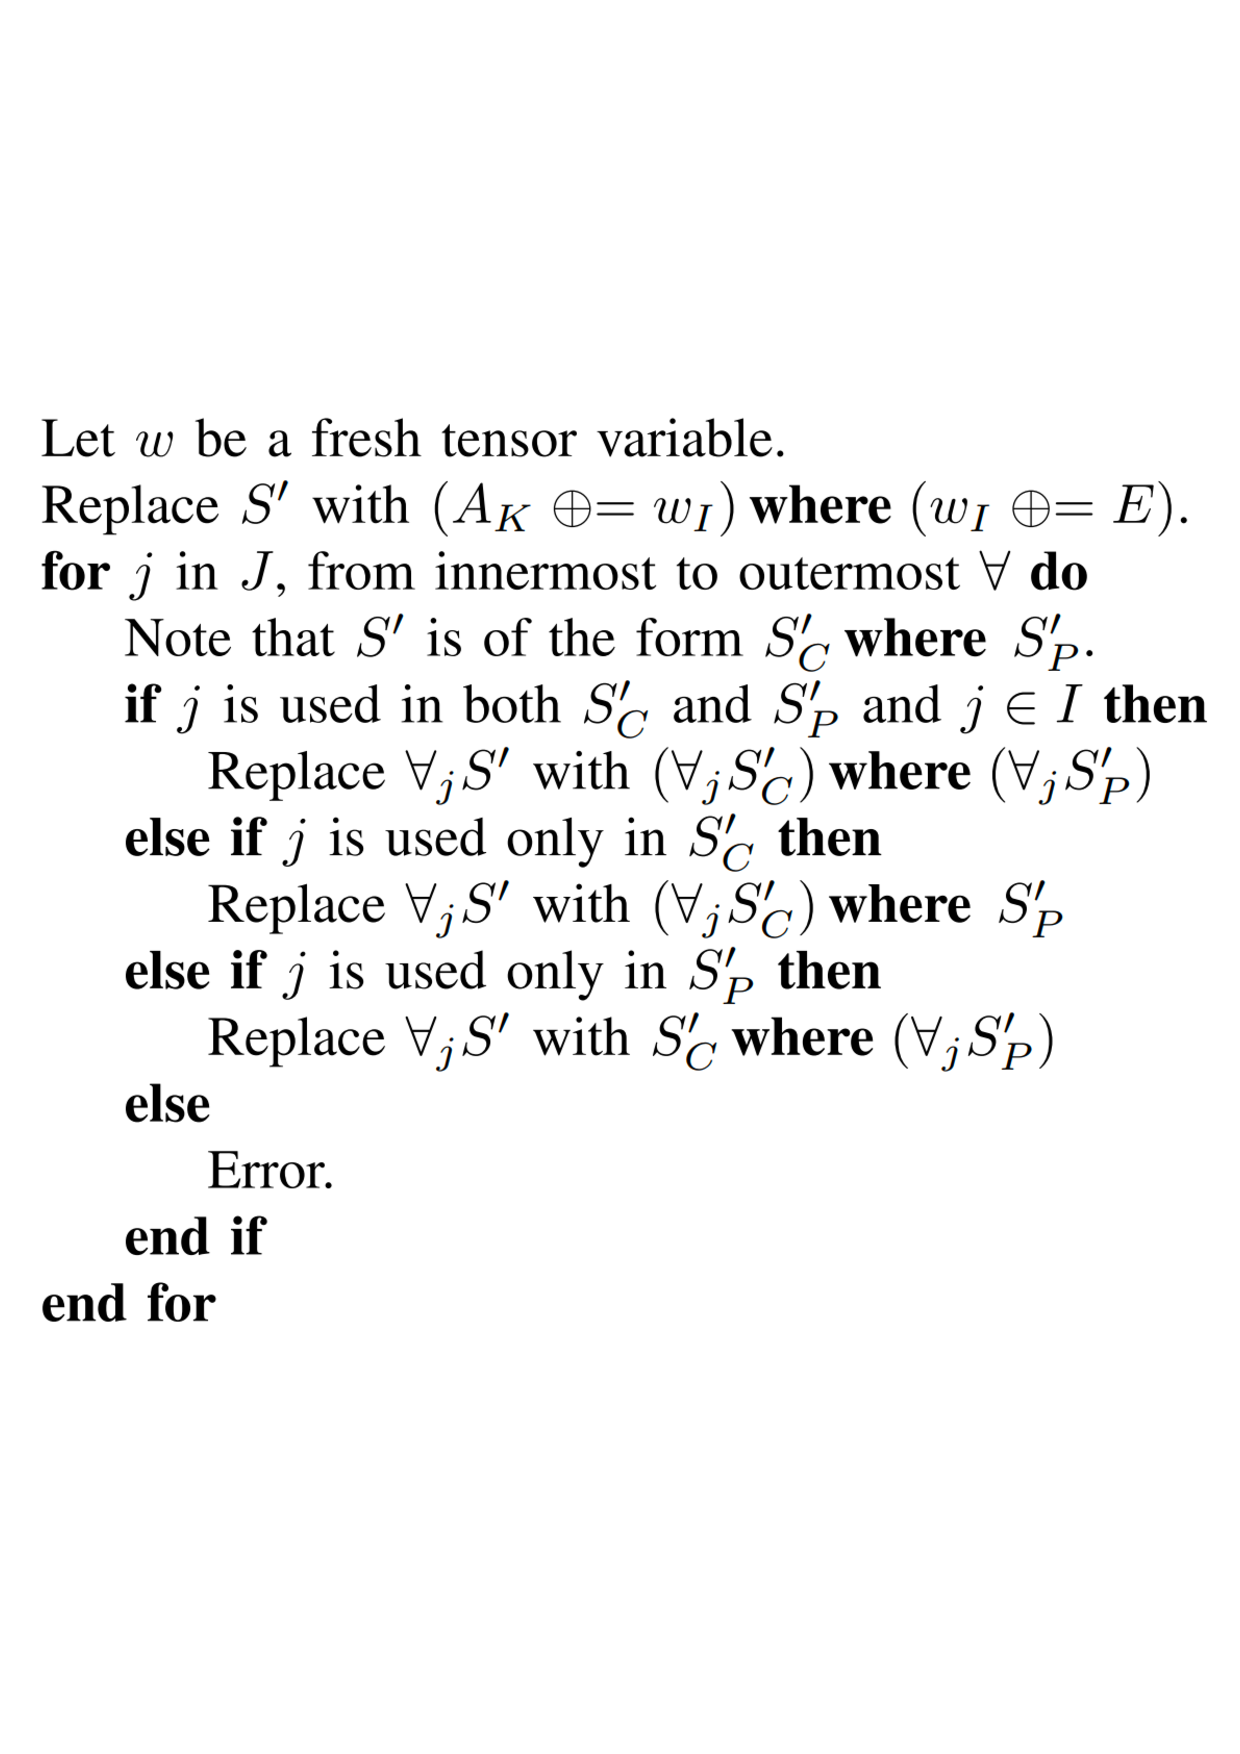
\includegraphics[width=0.5\linewidth]{workspace-algorithm.pdf}
  \caption{转移空间变换算法}
  \label{fig:workspace-transformation}
\end{figure}
三个转移空间变换的目标可以作为简单的启发式条件来描述算子在什么情况下会从转移空间变换中得到性能提升。假设$|$和$i$,且$i\subset I$。我们简单定义三种情况:
\begin{itemize}
  \item 简化合并。形如$(\forall_I A_i \oplus= B_I \otimes C_I \otimes D_I \otimes ...)$的表达式将超过3个稀疏张量$B,C,D,...$合并到稀疏张量$A$,会导致代价较大的合并。
  我们可以通过添加一个稠密转移空间,变换成 $(\forall_I A_i=w_i) where (\forall_I w_i \oplus= B_I \otimes C_I \otimes D_I \otimes ...)$ 
  \item 避免高代价的插入。形如$(\forall_I A_i \oplus= E_I)$的表达式中A是稀疏的,所以会积累到一个稀疏输出。可以通过稠密转移空间来避免稀疏插入,变换成$(\forall_I A_i = w_I) where (\forall_I w_I\oplus= E_I)$
  \item 提升循环不变代码。形如$(\forall_I A_I \oplus= E_I \otimes F_i)$的表达式会冗余计算表达式$F_i$。因此可以变换成$(\forall_I A_I \oplus= E_I \otimes w_i) where (\forall_i w_i = F_i)$
 \end{itemize} 
应用这些启发式条件可能需要先重写表达式,一个表达式不同等价形式的可能会导致有不同性能特征的表达式。

\section{编译}
\subsection{编译算法}
\begin{figure}
  \centering
  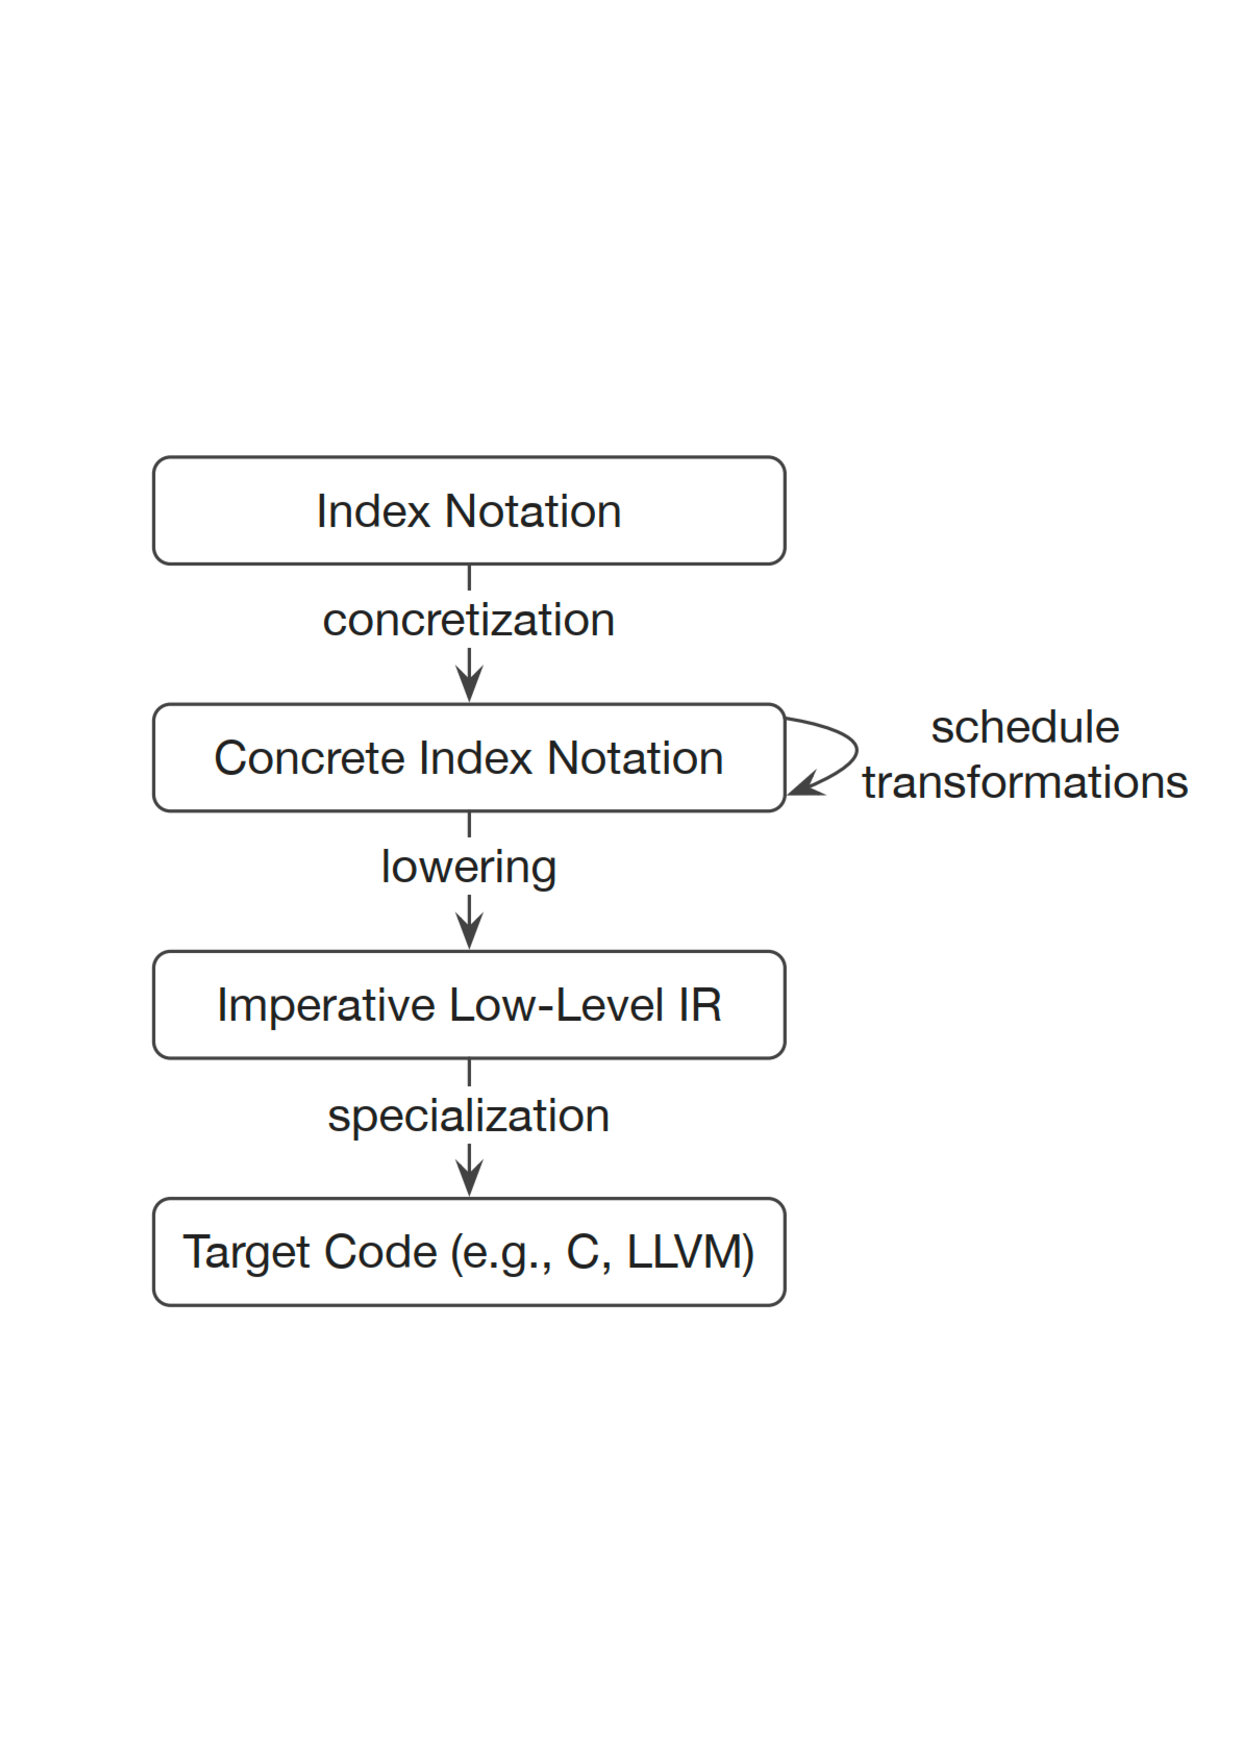
\includegraphics[width=0.5\linewidth]{Compilation-algorithm.pdf}
  \caption{编译变换算法}
  \label{fig:Compilation-transformation}
\end{figure}

\begin{figure}
  \centering
  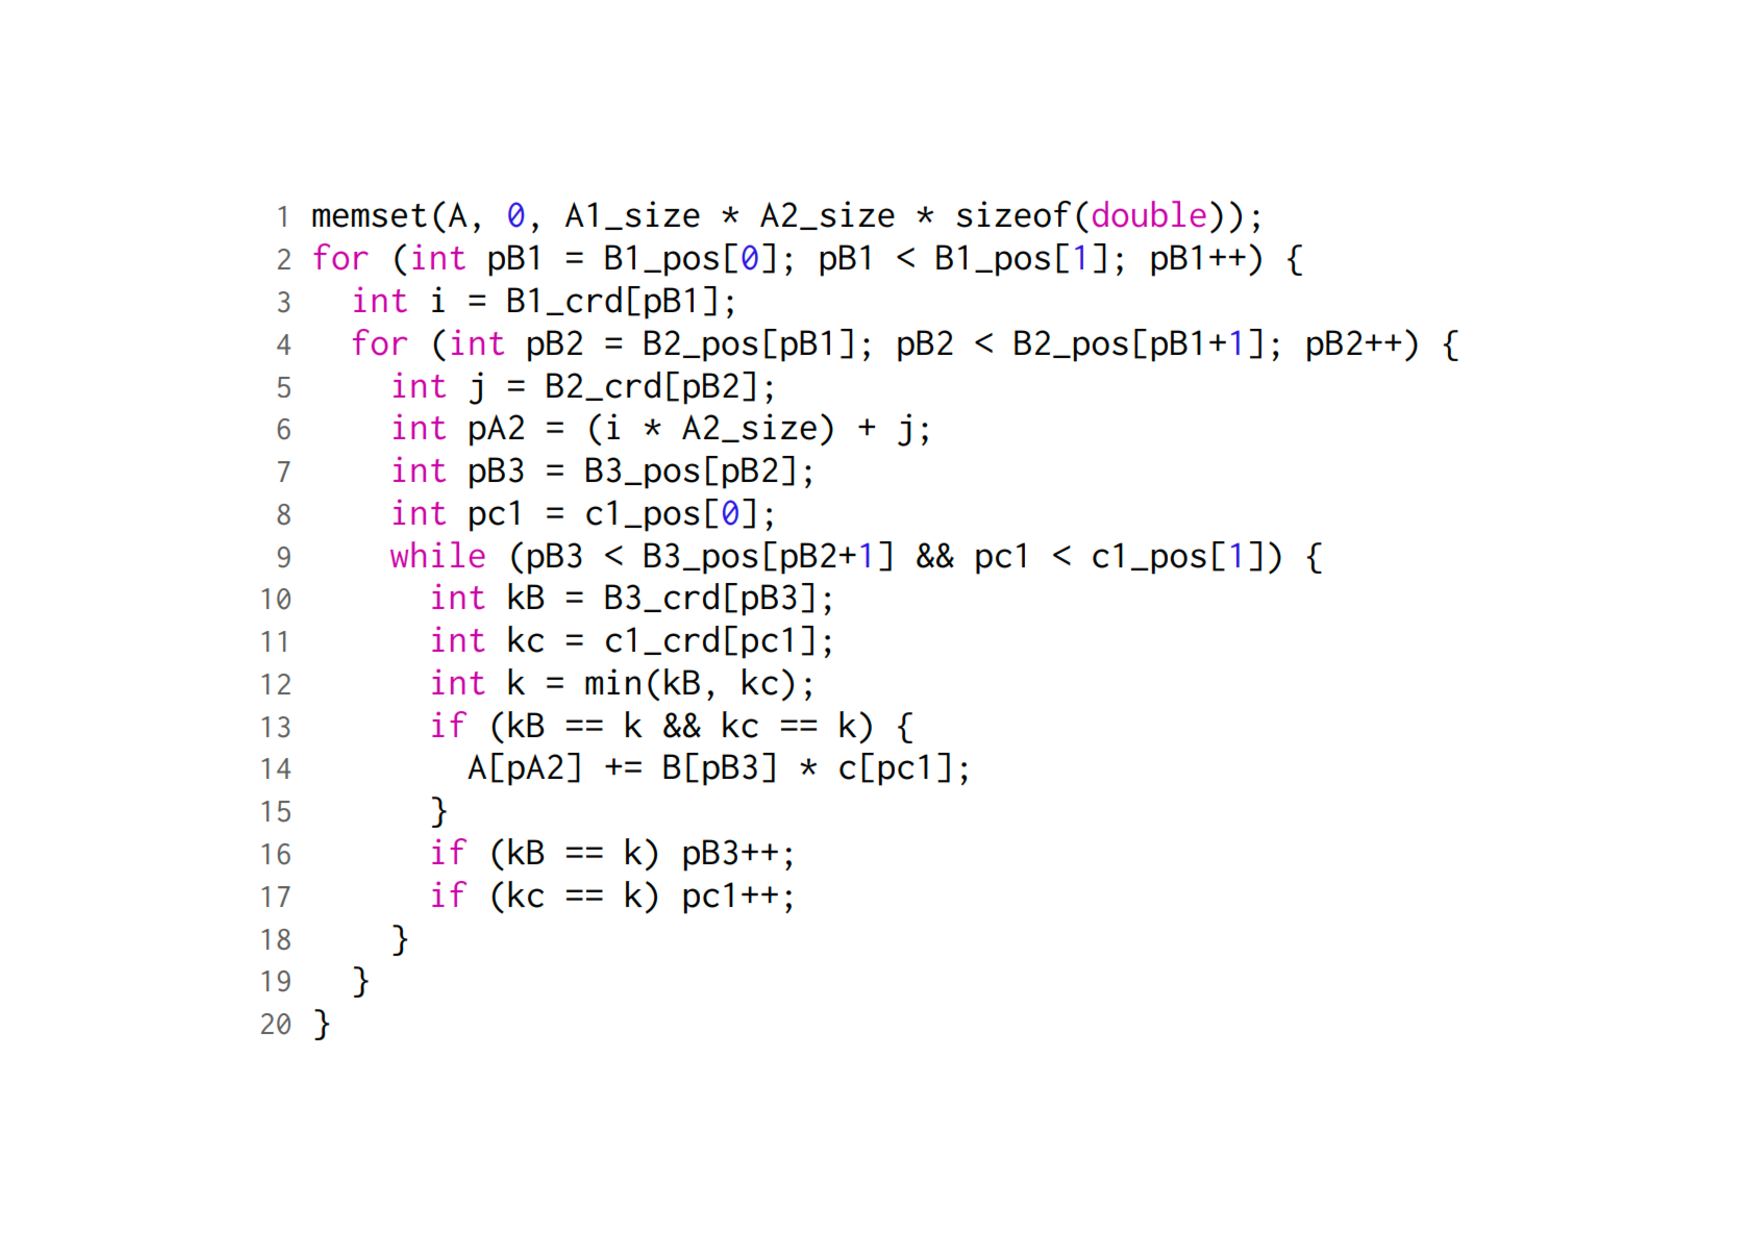
\includegraphics[width=0.5\linewidth]{sparse-vector.pdf}
  \caption{稀疏张量向量乘法代码}
  \label{fig:Sparse-vector}
\end{figure}

本节描述与具体索引符号之间的转换,称为具体化和降级。 图~\ref{fig:Compilation-transformation}显示了编译器工作流程,其中 IR 为方框,IR 转换为箭头。
大多数转换从较高抽象级别的 IR 转换为较低抽象级别的 IR。 然而,转移空间转换转换具体的索引表示法,这些转换是由用户或策略系统以编程方式请求的。 
具体化 IR 转换分两步将索引表示法转换为具体的索引表示法: 在索引表示法表达式中插入用于索引变量的 forall 语句。 
自由索引变量的 forall 语句嵌套在缩减变量的语句之外。 将 reduce 表达式替换为 where 语句,其生产者子语句减少为标量变量。 
结果是有效的具体索引表示法,可以通过转移空间转换进行优化,并进一步降低为低级稀疏命令式代码。 IR 降低将具体的索引符号转换为稀疏的命令式 C 类代码。 
该算法在内部使用我们在之前工作中描述的合并格,但比那里描述的代码生成算法更简单。 增加简单性的原因是它减少了具体的索引符号语句而不是迭代图。 
因此,它不需要在每个递归步骤中推断出哪些子表达式可用于发出。 代码生成算法在具体的索引符号语句上重复出现。 
当它遇到赋值语句时,它会将它们作为标量代码发出。 当遇到 where 语句时,算法会发出生产者端,然后是消费者端。 
最后,当它遇到序列语句时,它发出左侧,然后是右侧。 稀疏代码生成的主要复杂性与 forall 语句的代码生成隔离开来,因为它们必须同时在分层张量数据结构上进行迭代。 
我们建议读者参考我们之前的工作,以获得关于层次协同和迭代图图形符号的更多直觉。 在我们在本文中描述的代码生成方法中,迭代图已被具体的索引符号所取代。 
为了为 forall 语句生成代码,新的代码生成算法遍历 forall 的主体以收集由 forall 的索引变量索引的所有张量模式。 
为 forall 语句生成的代码必须通过协同处理它们的稀疏数据结构来协同处理这些张量模式。 例如,图~\ref{fig:Sparse-vector}显示了用于计算稀疏张量向量乘法的稀疏代码。 
为 i(第 2-3 行)和 j(第 4-5 行)的 forall 语句生成的外部循环仅迭代 B 的稀疏数据结构,因为 i 和 j 仅用于访问 B。
请注意,A 是一个 result 并且不需要迭代,因为根据定义,它的迭代空间与 B 相同。 
然而,为 forall 语句 k(第 9-12 行)生成的内部 while 循环在 B 的最后一个模式和向量 c 的稀疏数据结构上进行迭代。 
由于 B 和 c 相乘,因此 while 循环遍历它们的交集。 如果改为添加它们,则将生成三个 while 循环来共同处理它们的并集。
Forall 语句被降低为命令式代码,使用合并格生成合并代码。 我们建议读者将本说明限制在概述由于使用具体索引符号而导致的算法差异。 
然而,为具体索引符号子语句生成代码的递归调用的处理方式不同。 当在格点递归生成代码时,收集在该点耗尽的数据结构,并重写具体索引符号子语句以通过将它们象征性地设置为零来删除它们。 
因此,我们只对语句中未穷尽的部分进行复现,从而简化了算法。

在计算稀疏结果的代码列表中,到目前为止,我们只展示了计算结果而不组装稀疏索引结构的算子。这让我们可以专注于循环结构,而不会增加转移空间组装的复杂性。
此外,在数值代码中,将组装索引结构(通常称为符号计算)的内核与计算值(数值计算)的内核分开是很常见的。 
我们在之前的工作中概述并在此处修改的代码生成算法可以发出,或者一个同时组装结果索引结构并计算其值的算子。 
当从具体索引符号生成汇编内核时,一个转移空间会产生两个数组,它们一起跟踪转移空间的非零坐标。 
第一个数组(例如,行列表)是已插入到转移空间中的坐标列表,第二个数组(例如,行)是一个布尔数组,用于防止向坐标列表中进行冗余插入。 
图~\ref{fig:assembly-code}显示了稀疏矩阵乘法示例的线性组合的汇编代码。 将转移空间复制到 A 的循环开始于第 32 行。在计算算子中,A 的索引结构已预先组装,
因此代码生成算法会发出循环以迭代 A。然而,在汇编内核中,它会发出代码以迭代转移空间的索引结构。 
此外,汇编内核在第 15-18 行插入转移空间索引(行列表),而不是计算结果,并在第 23 行对索引列表进行排序,以便对 A 的新行进行排序。 
请注意,排序是可选的,只有在必须对结果进行排序时才需要。 最后,汇编内核通过重复加倍在第 26-29 行分配额外的坐标内存。
\begin{figure}
  \centering
  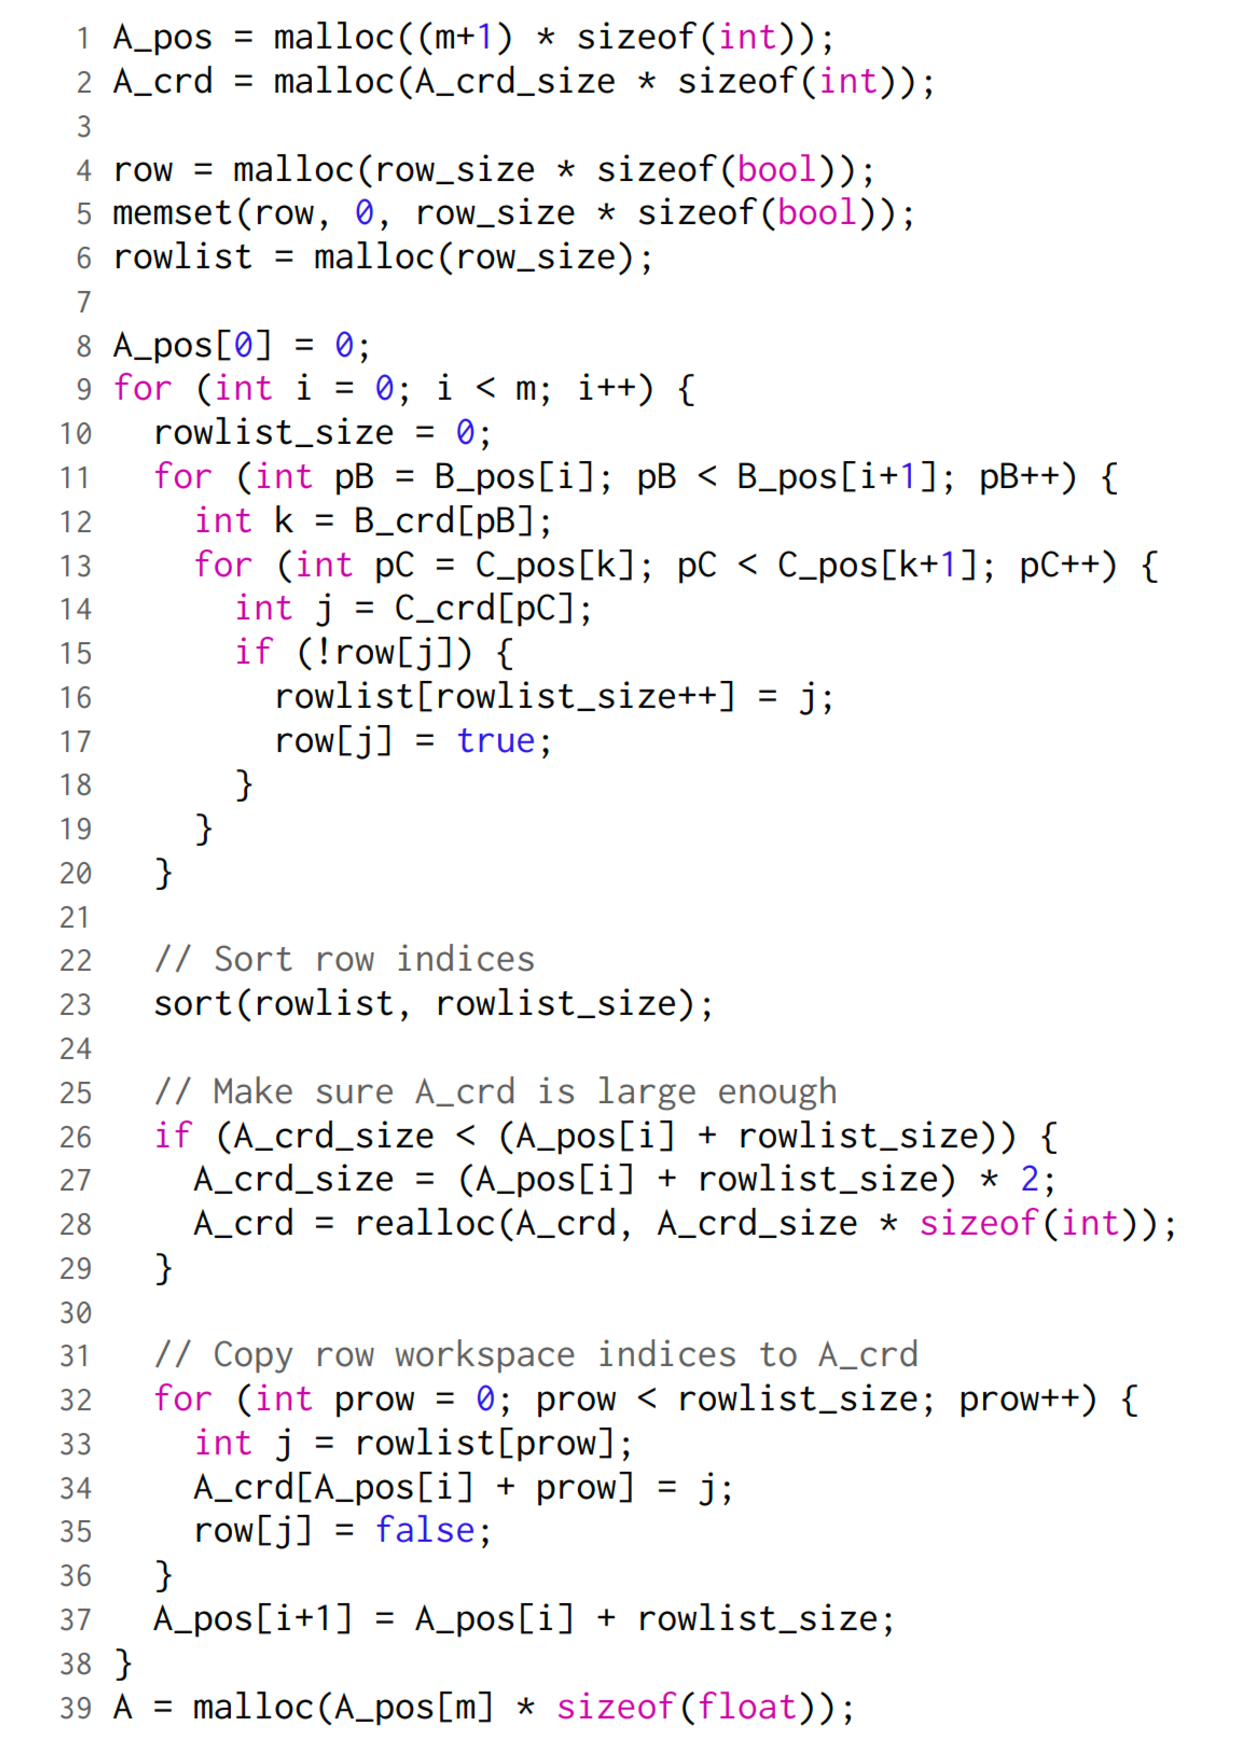
\includegraphics[width=0.5\linewidth]{assembly-code.pdf}
  \caption{汇编代码}
  \label{fig:assembly-code}
\end{figure}

\subsection{案例分析}
矩阵化的张量乘Khatri-Rao积(MTTKRP)在变换最小二乘(ALS)算法中是关键算子。ALS用于计算张量的典范多边体分解(CPD)。
CPD分解是矩阵SVD分解的高维形式,并且在数据分析,机器学习,神经科学,图片分类和压缩以及其他领域中都有广泛应用。
ALS算法和MTTKRP算子可以被用来分解任意维度的张量。对于k维度张量分解的MTTKRP算子由一个k维度张量在不同维度乘k-1个矩阵。例如,四维MTTKRP算子是$A_{ij} = \sum_{klm}B_{iklm}C_{mj}D_{lj}E_{kj}$。
这个部分我们向3维MTTKRP算子应用两次转移空间变换来优化。但是,相同的变换也可以应用在更高维度的算子。MTTKRP算子的第一个转移空间优化基本上等效于SPLATT库中的算法,但是第二个变换让MTTKRP可以写入稀疏输出。
用张量索引符号表达3维MTTKRP算子为
\begin{equation*}
  A_{ij} = \sum_{kl} B_{ikl}C_{lj}D_{kj}
\end{equation*}
MTTKRP最简单的具体索引符号表达形式为
\begin{equation*}
  \forall_{iklj} A_{ij} += B_{ikl}C_{lj}D_{kj}
\end{equation*}
在这个表达形式中forall语句从初始具体形式中变换顺序得到,所以稀疏张量B按照稀疏层级结构的顺序访问。当我们向$B_{ikl}C_{lj}$在j维度应用转移空间变换时得到
\begin{equation*}
  \forall_{ik} (\forall_j A_{ij}+=w_j D_{kj})\, \mathbf{where}\, (\forall_{lj} w_j +=B_{ikl}C_{lj})
\end{equation*}
这个转移空间变换将forall语句中j这一角标变量分裂到where语句两侧的forall语句中。注意l变量没有被消费者中的任何张量利用,因此包含l的语句在消费者中被删除了。这个循环的删除是我们应用转移空间变换的目标
因为这可以导致$w_jD_{kj}$可以在更高的层级计算。这也展示了转移空间变换可以被用来在稀疏代码中提升循环不变的代码。
\begin{figure}
  \centering
  \subcaptionbox{MTTKRP的第一个转移空间变换\label{fig:mttkrp-a}}
    {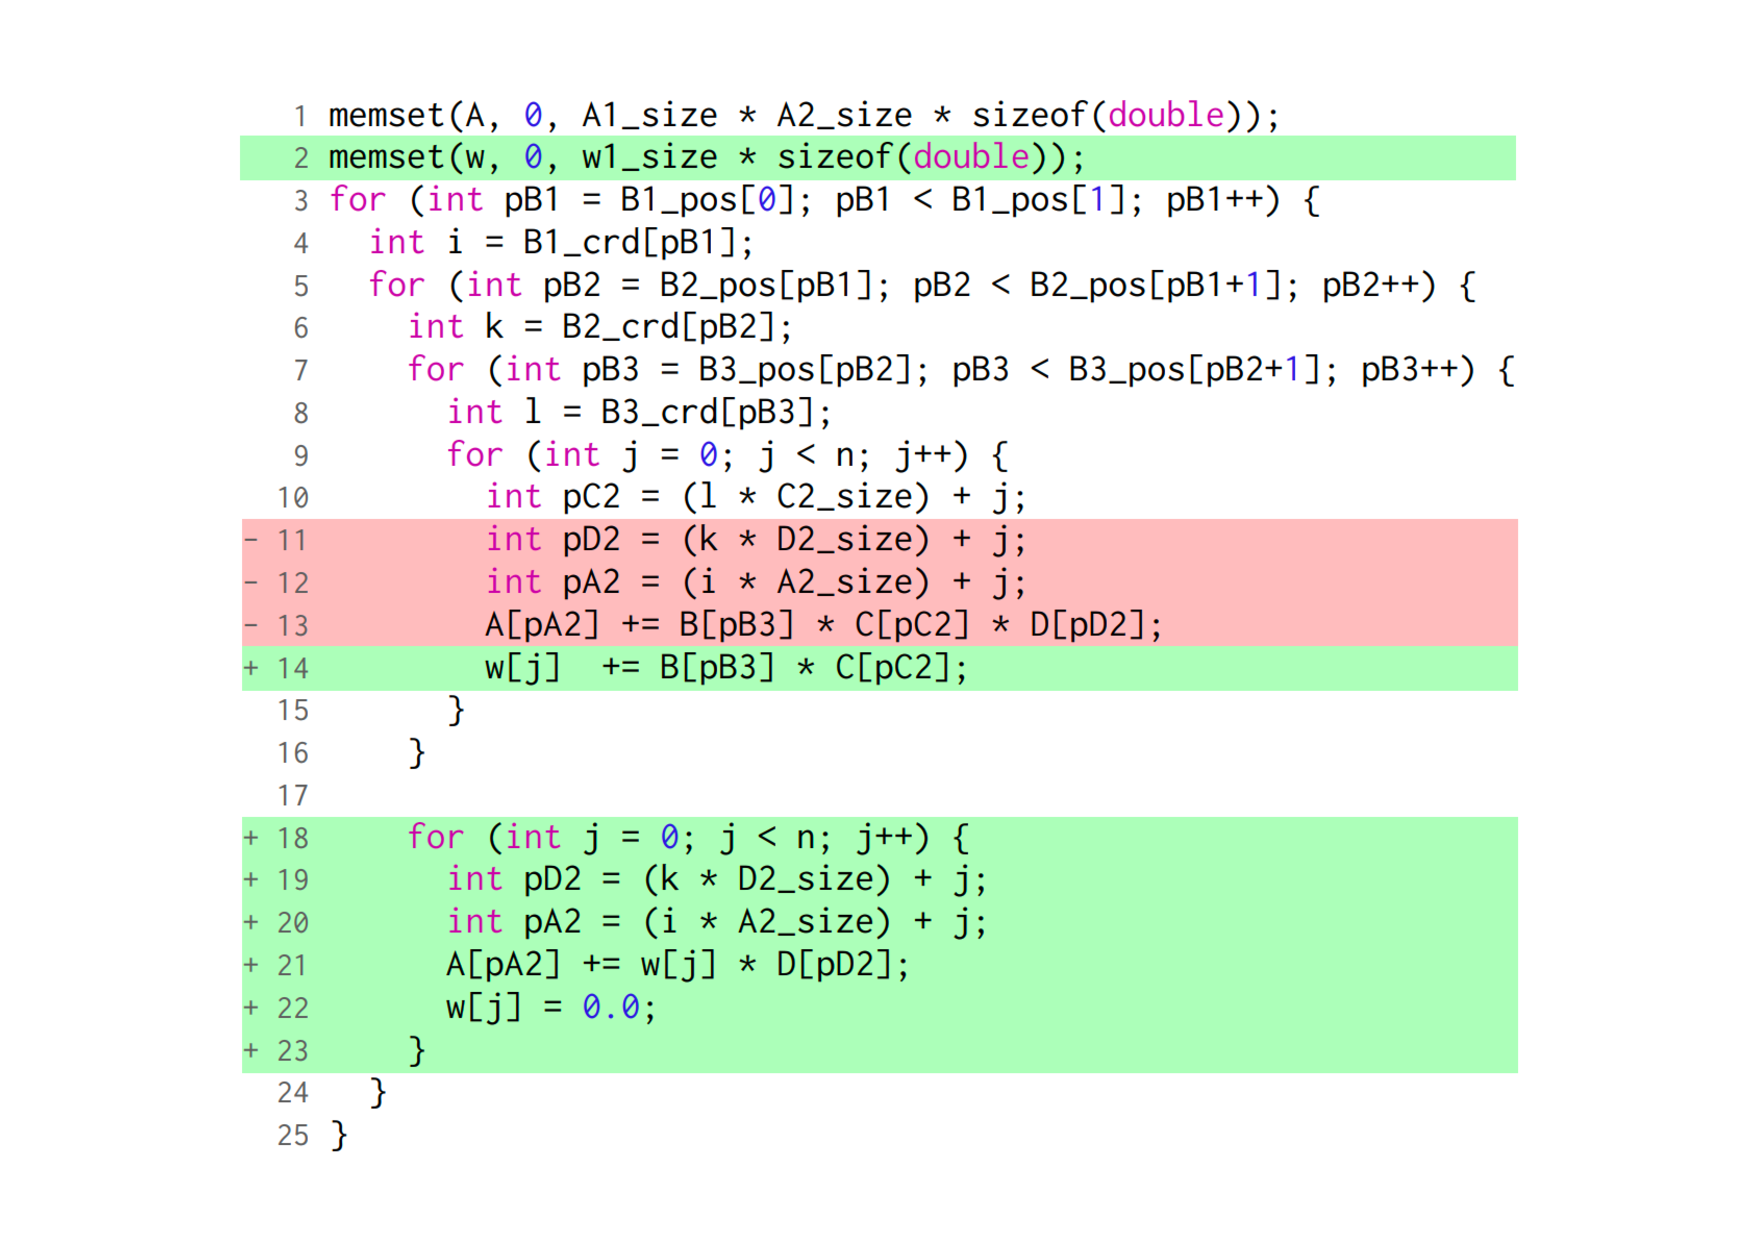
\includegraphics[width=0.35\linewidth]{MTTKRP-1.pdf}}
  \subcaptionbox{MTTKRP的第二个转移空间变换\label{fig:mttkrp-b}}
    {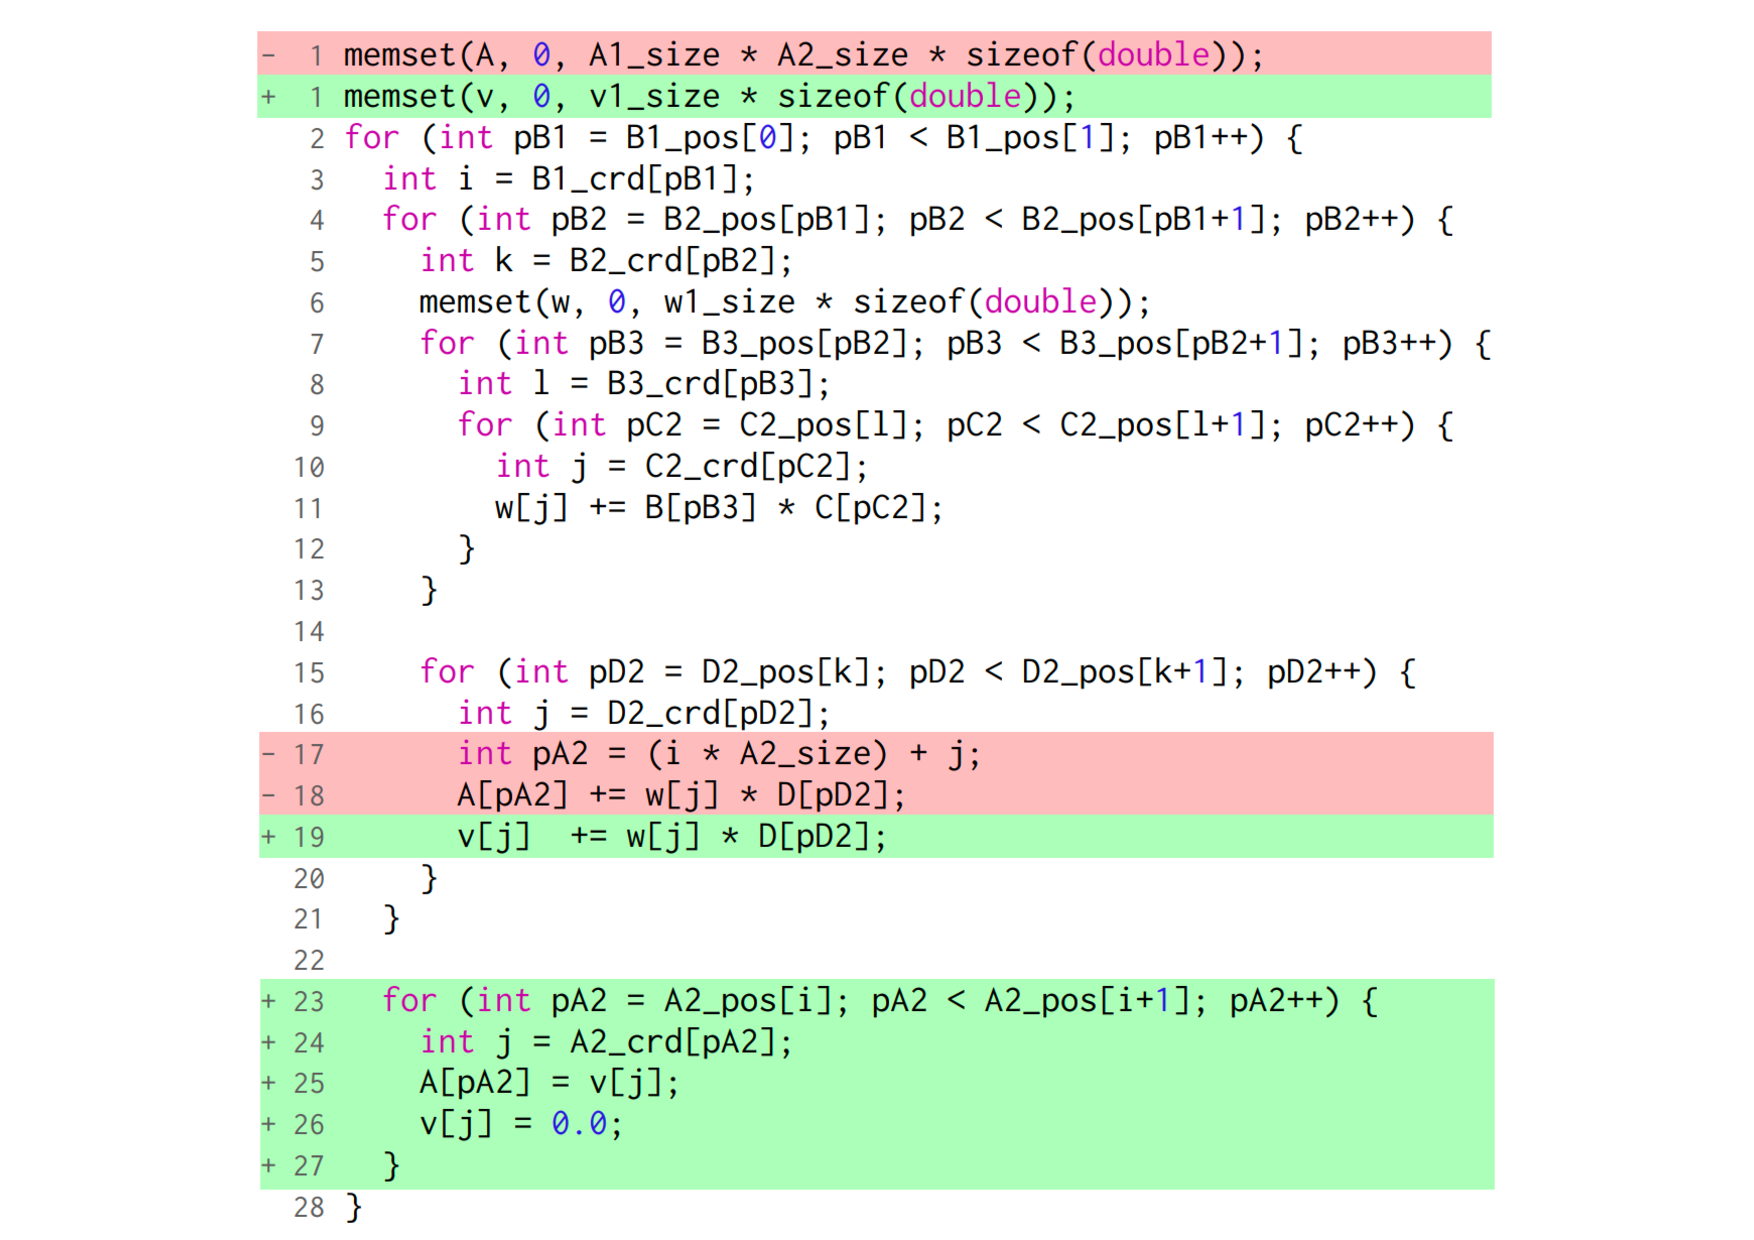
\includegraphics[width=0.35\linewidth]{MTTKRP-2.pdf}}
  \caption{3维MTTKRP}
  \label{fig:mttkrp-code}
\end{figure}
图~\ref{fig:mttkrp-a}中的源代码差异显示了第一个转移空间转换对编译具体索引符号表达式所产生的稀疏代码的影响。 白色背景显示未更改的代码,红色背景显示已删除的代码,绿色背景显示添加的代码。 转换后的具体索引符号生成的代码中,
从第 9 行开始的 j 循环(将 B 与 D 相乘)已从第 7 行开始的 l 循环中移除,从而减少了乘法运算。 代价是转移空间减少了时间局部性,因为写入值和读回它们之间的重用距离。 
实验结果表明,这种特定的转换可以提高两个大型数据集的性能,并降低较小数据集的性能,因此应谨慎应用。
MTTKRP算子会向结果矩阵A中随机写入值。我们可以从累计额的赋值表达式$A_{ij}+=w_j D_{kj}$中观察到这一特征。原因是这个声明在一个或多个forall循环中,并且是一个累加操作。如果A是稀疏的,那么插入就会代价很高。所以,代码性能又会因为应用的转移空间变换而提升。
这次变换为提前在转移空间v中计算$w_jD_{kj}$。得到如下表达式
\begin{equation*}
  \forall_{i} (\forall_j A_{ij}=v_{j})\, \mathbf{where}\, (\forall_k(\forall_j v_j += w_j D_{kj})\mathbf{where}\, (\forall_{lj} w_j +=B_{ikl}C_{lj}))
\end{equation*}
因此,对 A 的赋值不再是递增赋值。 相反,这些值被分散到一个具有随机访问权限的密集转移空间中,然后在计算完一整行结果后复制到结果中。 图~\ref{fig:mttkrp-b}中的源代码差异显示了在转移空间 v 中
生成结果矩阵 A 稀疏和预计算 $w_jD_{kj}$ 对编译代码的影响。转换前的代码(红色)和转换后的代码(绿色)均采用操作数矩阵 C 和 D 是稀疏的,
与图~\ref{fig:mttkrp-a}中的 C 和 D 是密集的相反。 与稀疏矩阵乘法代码一样,转移空间变换后的代码分散到一个密集的转移空间 v 中,
并且在计算出整行后,将转移空间非零值附加到结果中。

\section{性能评估}
在本节中,我们通过将带有转移空间的稀疏内核的性能与用于线性和张量代数的手写最先进的稀疏库的性能进行比较来评估转移空间转换的有效性。
\subsection{实验方法}
所有实验都在双插槽 2.5 GHz Intel Xeon E5-2680v3 机器上运行,该机器具有 12 个内核/24 个线程和每个插槽 30 MB 的 L3 缓存,运行 Ubuntu 14.04.5 LTS。 该机器包含 128 GB 内存并运行内核版本 3.13.0 和 GCC 5.4.0。 对于所有实验,除非另有说明,否则我们确保机器处于空闲状态并报告单线程执行的平均冷缓存性能。
我们通过比较线性代数算子与 Eigen 和 Intel MKL 2018.0 这两个高性能线性代数库的性能来评估我们的方法。 我们还将张量代数内核的性能与用于稀疏张量分解的高性能 SPLATT 库进行了比较。 我们从 SuiteSparse Matrix Collection 和 FROSTT Tensor Collection 中获得了用于实验的真实矩阵和张量。 图~\ref{fig:tensor-info}显示了实验中使用的矩阵和张量的详细信息
\begin{figure}
  \centering
  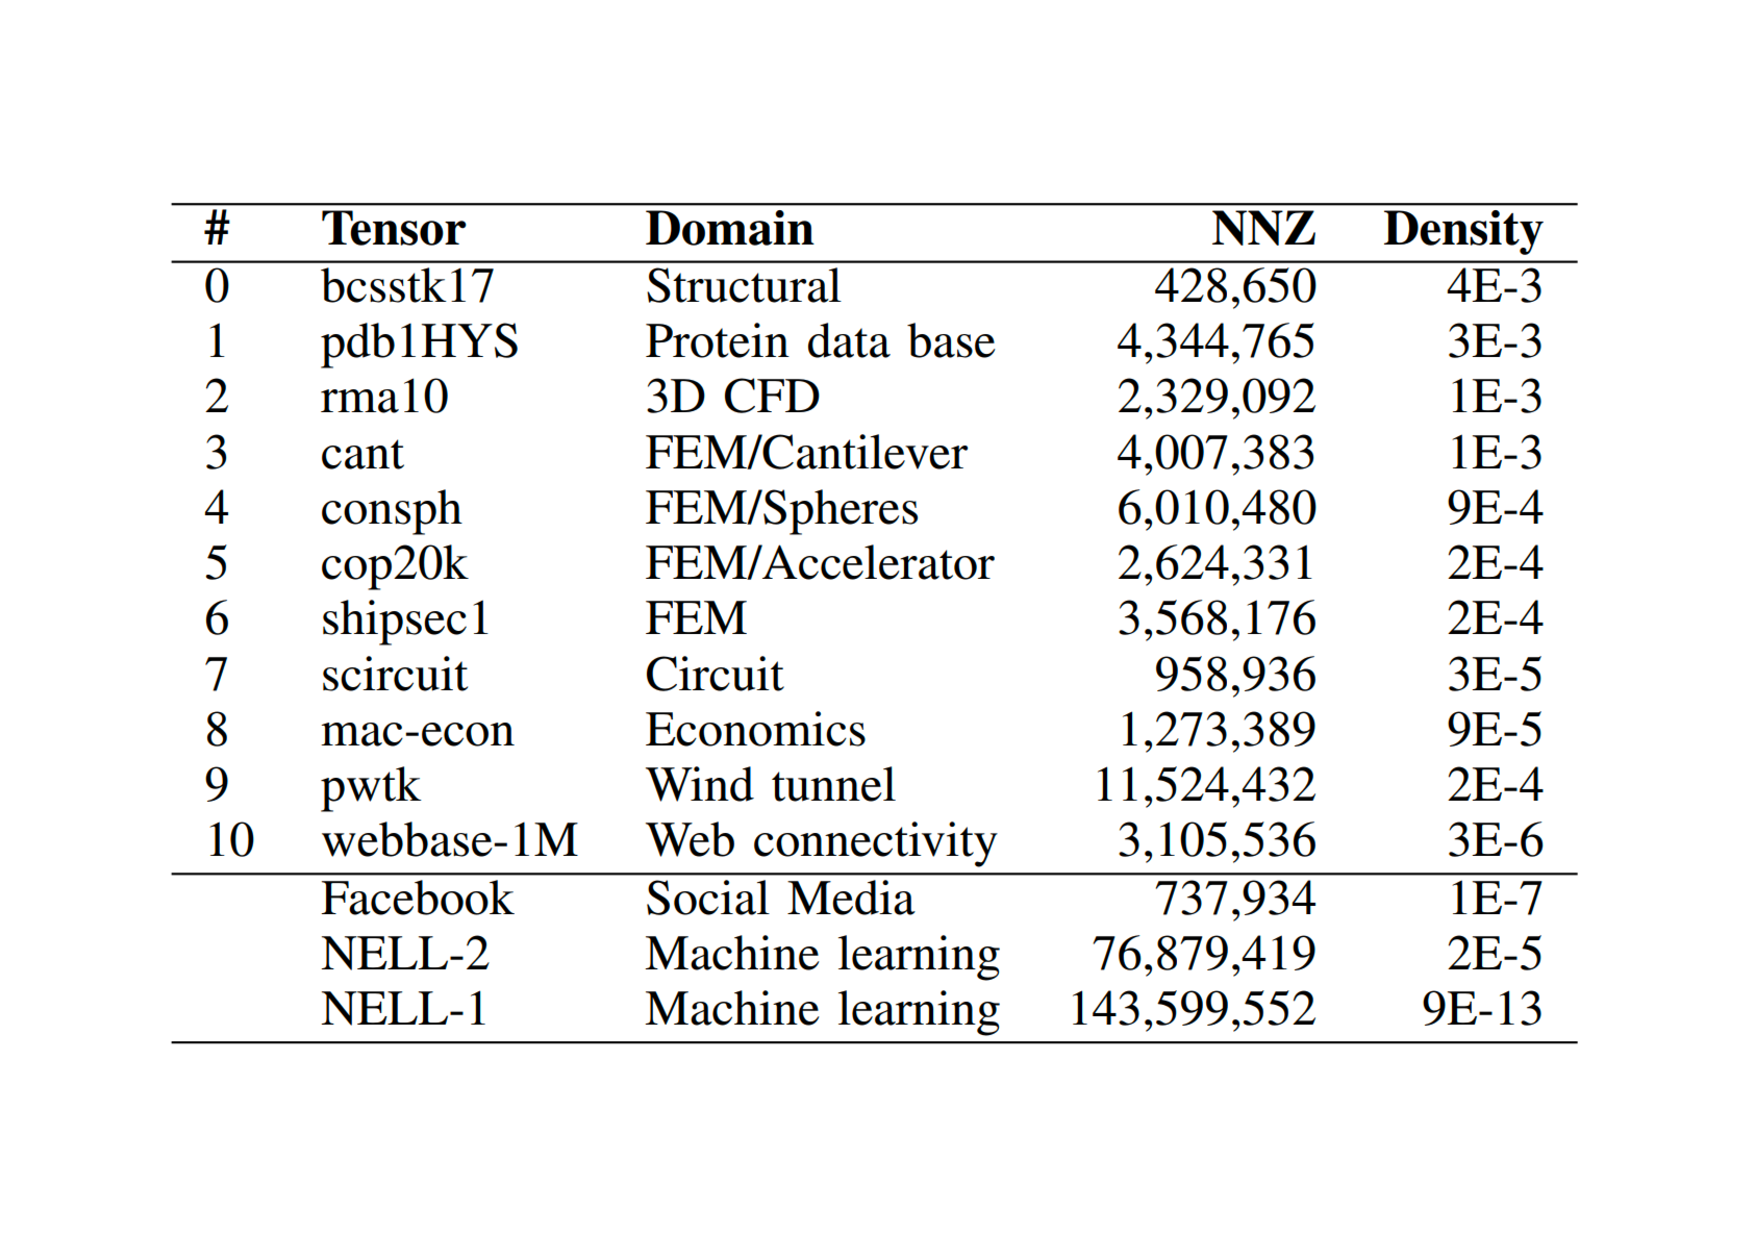
\includegraphics[width=0.5\linewidth]{tensor-info.pdf}
  \caption{实验张量信息}
  \label{fig:tensor-info}
\end{figure}
\subsection{稀疏矩阵乘法}
\begin{figure}
  \centering
  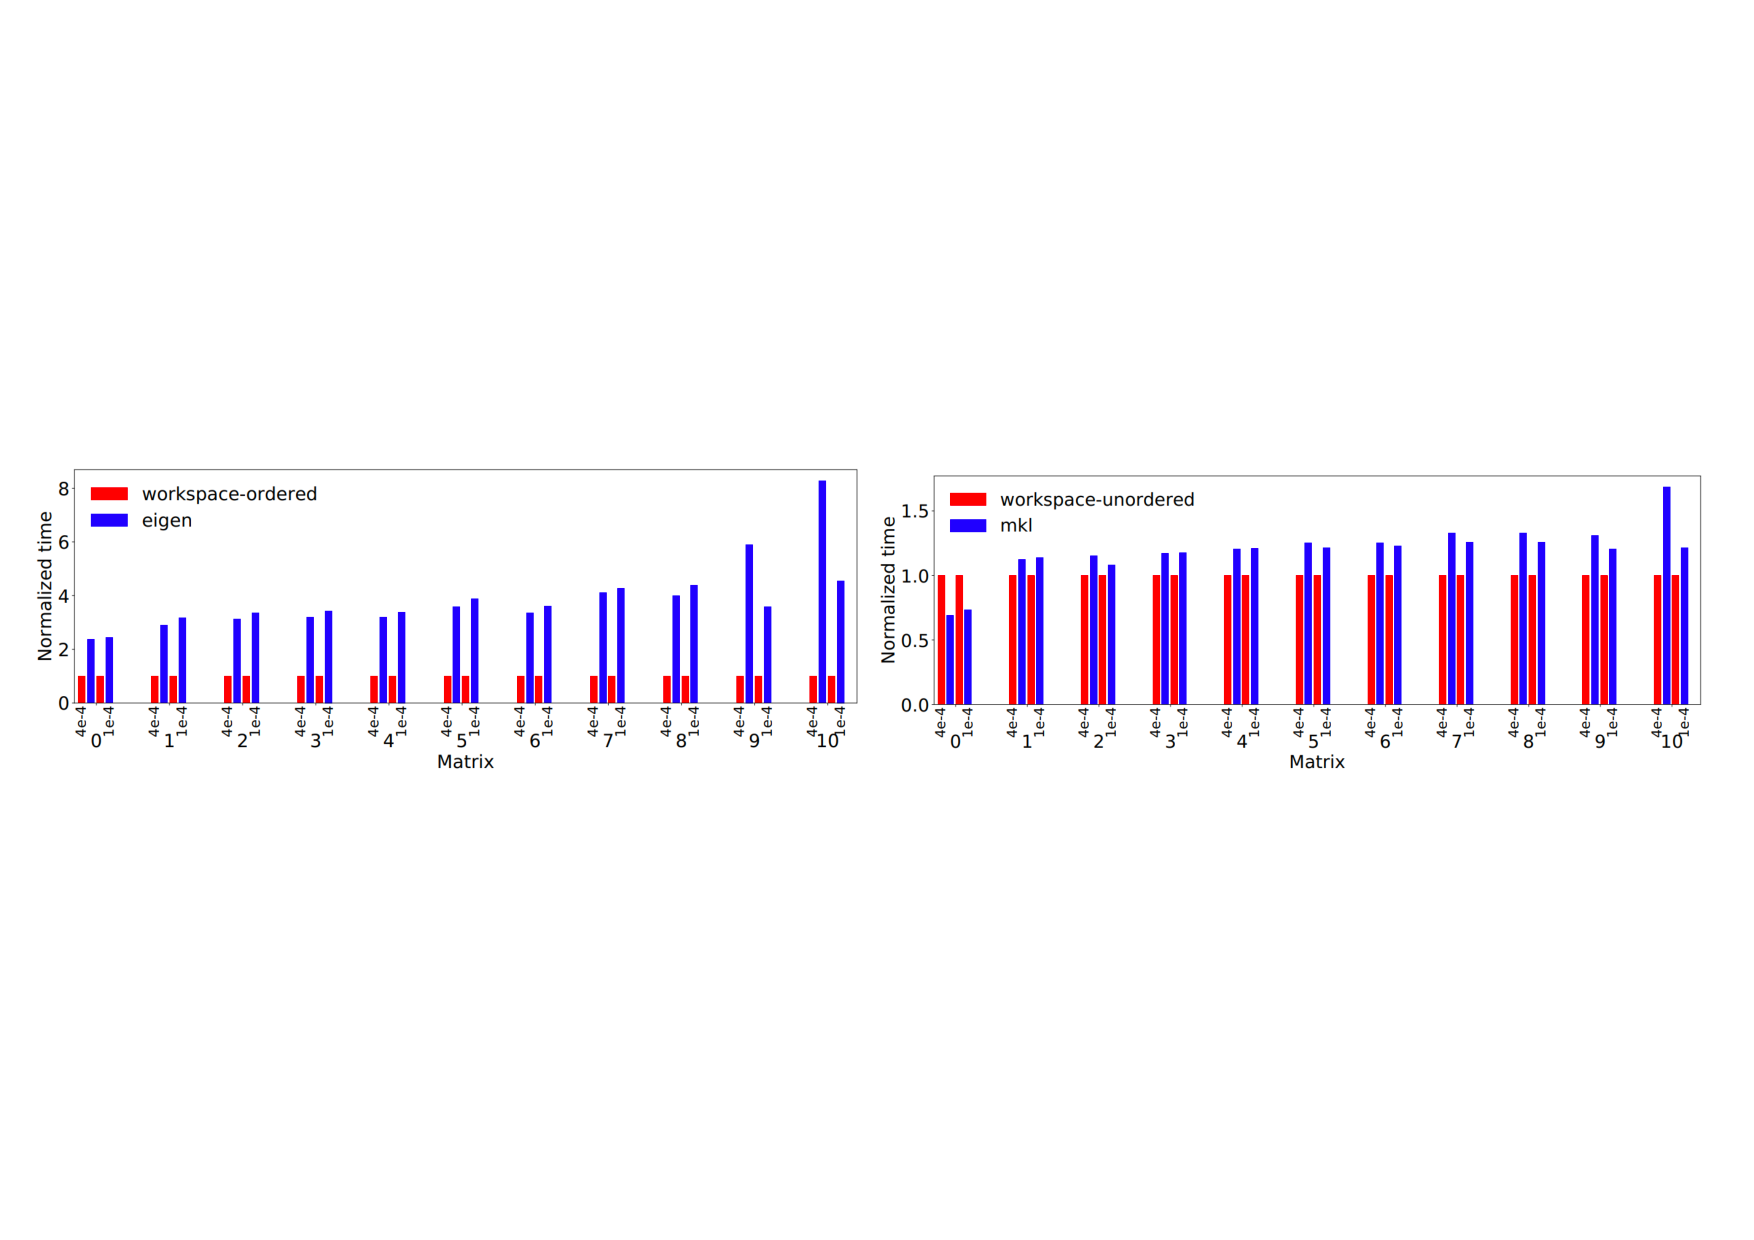
\includegraphics[width=0.5\linewidth]{all-results.pdf}
  \caption{稀疏矩阵乘法实验结果}
  \label{fig:all-results}
\end{figure}
\begin{figure}
  \centering
  \subcaptionbox{3维MTTKRP实验结果\label{fig:mttkrp-results}}
    {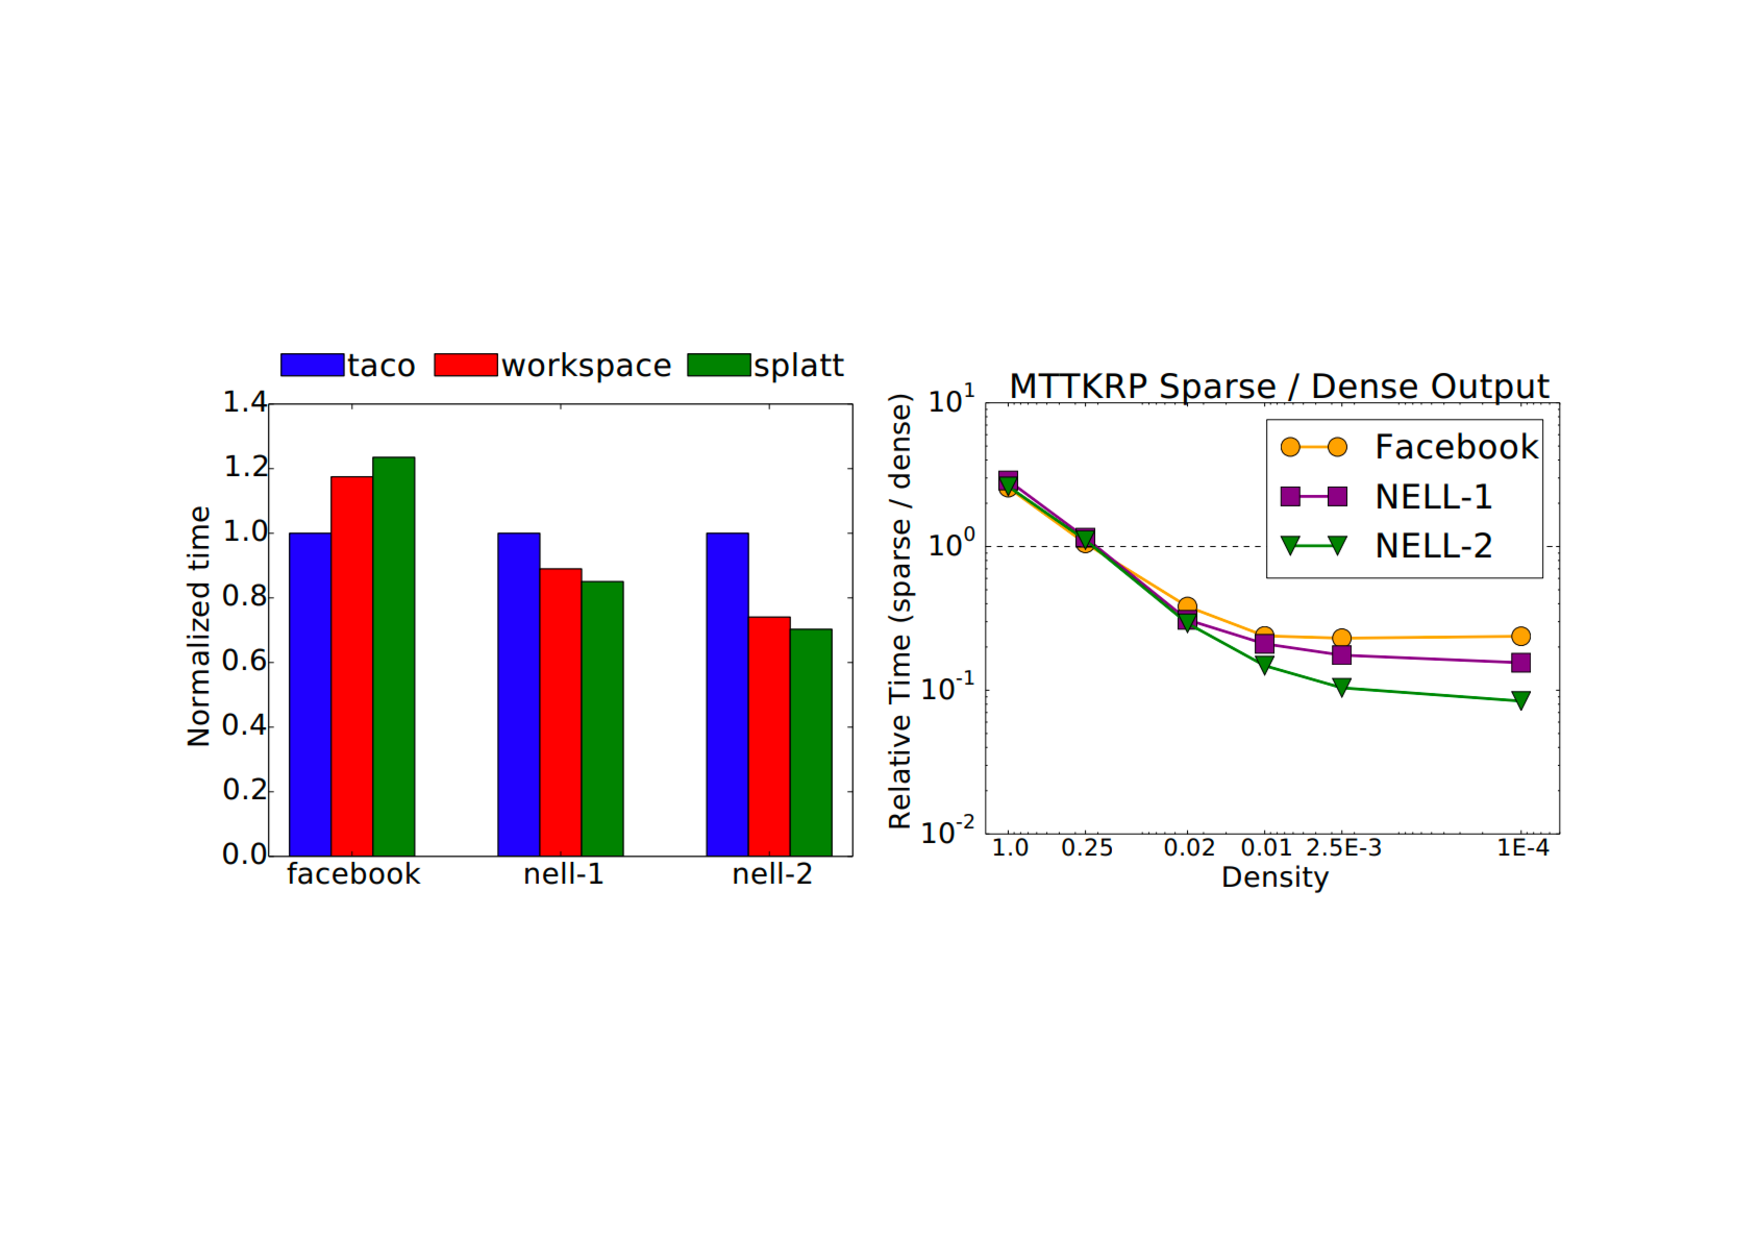
\includegraphics[width=0.35\linewidth]{mttkrp-results.pdf}}
  \subcaptionbox{3维张量加法实验结果\label{fig:spadd-results}}
    {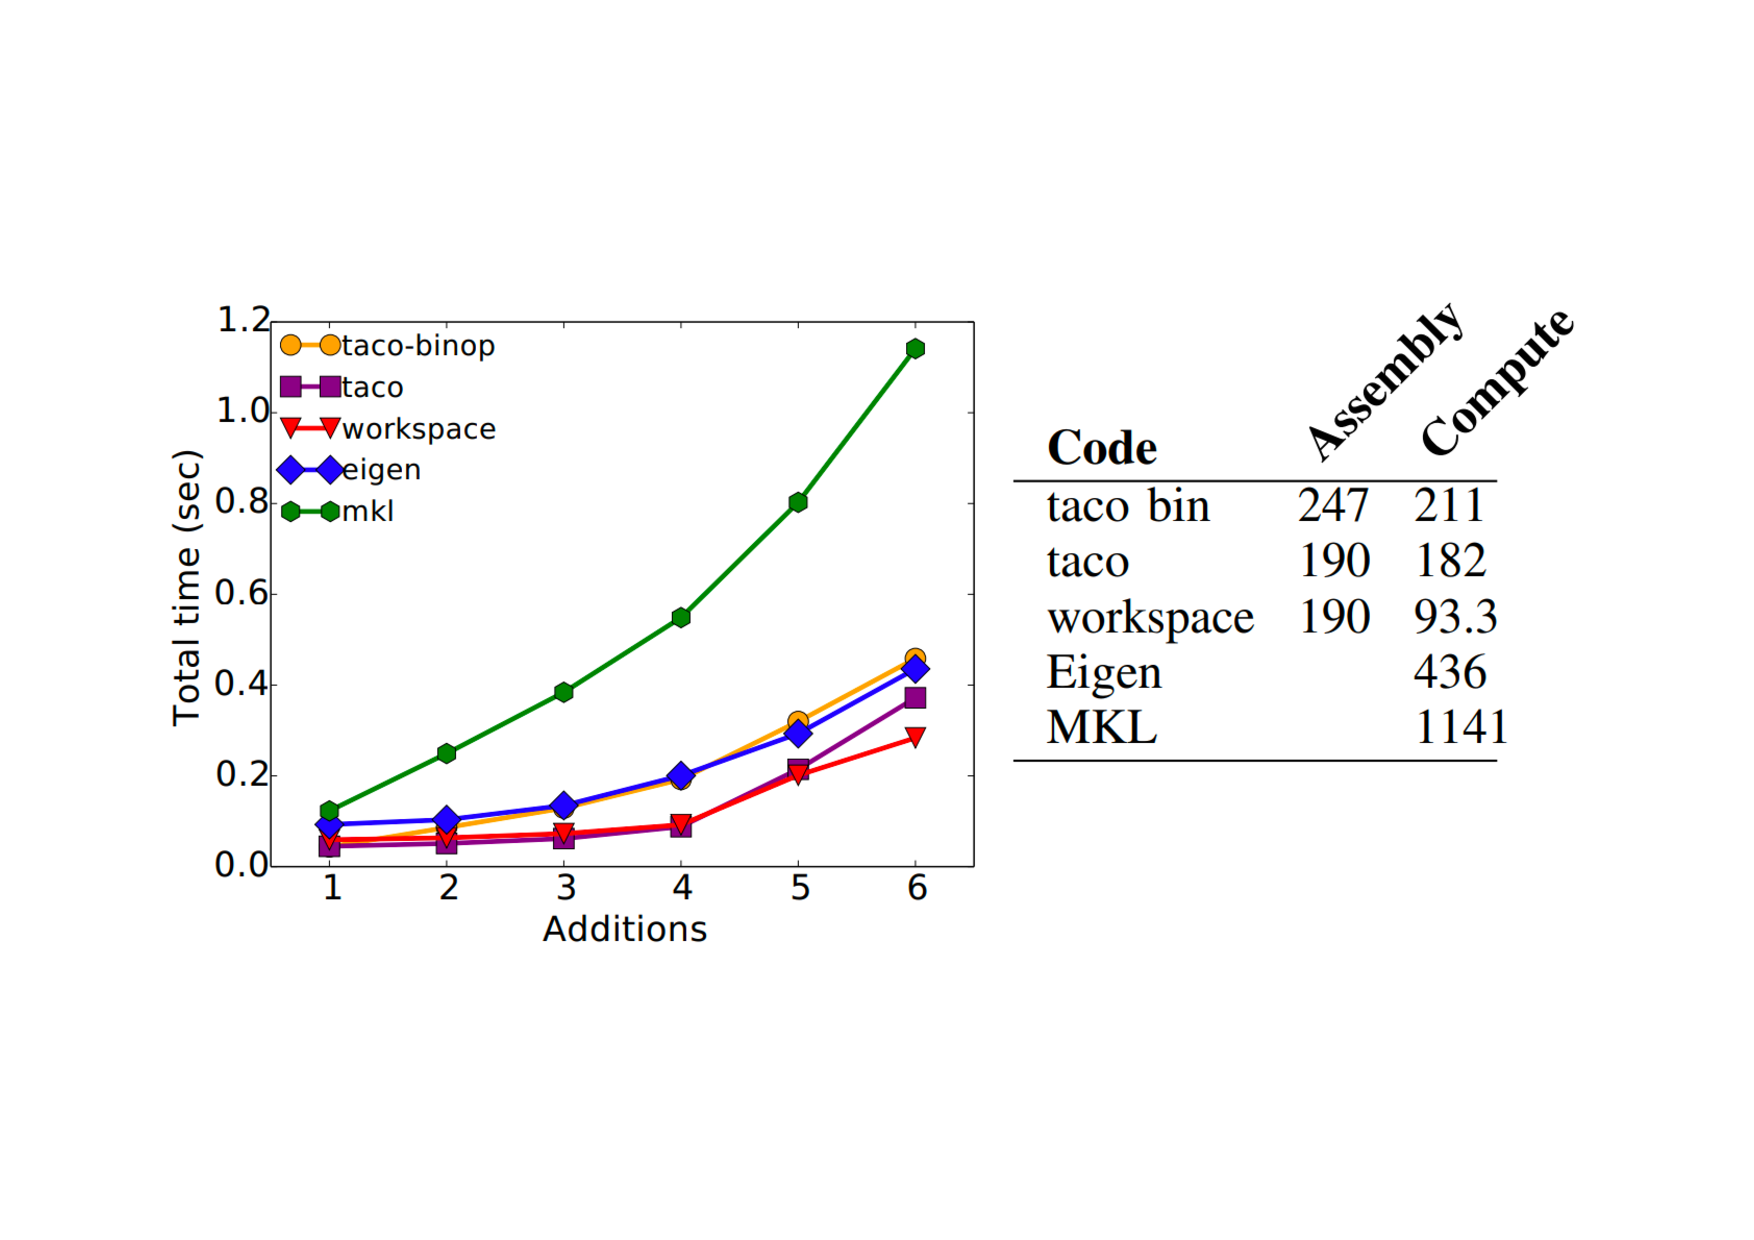
\includegraphics[width=0.35\linewidth]{spadd-results.pdf}}
  \caption{MTTKRP和张量加法实验结果}
  \label{fig:other-results}
\end{figure}

快速稀疏矩阵乘法算法使用转移空间来存储中间值。 我们将生成的转移空间算法与 MKL 和 Eigen 中的实现进行比较。 我们使用两个操作数计算稀疏矩阵乘法:图~\ref{fig:tensor-info}中的真实矩阵和使用特定目标稀疏性和均匀随机非零位置生成的合成矩阵。 Eigen 实现了一种排序算法,该算法对每一行中的列条目进行排序,因此它们是有序的,而 MKL 的 mkl sparse spmm 实现了一种未排序的算法——列条目是未排序的。
因为这两种算法产生不同的成本,我们将其与转移空间变体进行比较每个; 对于排序算法,我们包括排序时间。 在这两种情况下,转移空间算法都将输出矩阵的组装与计算融合在一起。 
请注意,我们之前的实现不会生成稀疏矩阵,因为它不支持插入到稀疏结果中,因此我们在此比较中省略了它。 图~\ref{fig:all-results}显示了图~\ref{fig:tensor-info}中每个矩阵的稀疏矩阵乘法乘以非零密度 1E-4 和 4E-4 的合成矩阵的运行时间,使用我们的转移空间实现。 
平均而言,Eigen 比我们的方法慢,后者生成 Gustavson 矩阵乘法算法的变体,对于两个稀疏度级别分别慢 4 倍和 3.6 倍。 
对于未排序的算法,我们与 MKL 进行比较,发现我们的性能平均快 28\% 和 16\%。 生成的转移空间算法比 MKL 的手动优化实现更快(最多 68\%),只有一种情况除外,后者慢 31\%。

矩阵化张量乘积 Khatri-Rao 积 (MTTKRP) 用于计算数据分析中的张量分解。 三维版本将一个稀疏 3 张量和两个矩阵作为输入,并输出一个矩阵。 图~\ref{fig:mttkrp-results}显示了我们的转移空间算法在三个输入张量上的结果,
与 taco 和手动编码的 SPLATT 库进行了比较。 我们比较并行单套接字实现,使用 numactl 将执行限制在单个套接字。
对于 NELL-1 和 NELL-2 张量,转移空间算法分别优于 taco 中基于合并的算法 12\% 和 35\%,并且与 SPLATT 的手动编码性能相差不到 5\%。 在较小的 Facebook 数据集上,合并算法比我们的实现和 SPLATT 的都快。 
不同的输入在不同的算法下表现更好,这证明了能够生成两个版本的算法的优势。 由于 MTTKRP 是广泛使用的交替最小二乘张量分解算法的最大瓶颈,占计算时间的 69-99\%,我
们预计使用转移空间变换加速 MTTKRP 将为整体张量分解运行时间提供类似的加速。

支持张量和矩阵操作数都是稀疏的MTTKRP也非常有用,如果结果也是稀疏的,则 MTTKRP 可以更快,因为它只需要迭代非零值。 然而,代码很难编写,并且不能由当前版本的 taco 生成。 在本节中,我们评估稀疏 MTTKRP 的转移空间实现。 
因为我们没有实现具有稀疏输出的 MTTKRP 的并行版本,所以我们与两个 MTTKRP 版本的单线程实现进行比较。 哪个版本更快取决于稀疏操作数的密度。图~\ref{fig:mttkrp-results}显示了比较具有稀疏矩阵的 MTTKRP 与具有密集矩阵的
MTTKRP 的计算时间的实验,因为我们改变了随机生成的输入矩阵的密度。 对于每个张量,交叉点大约为 25\% 的非零值,这表明即使输入中只有适度的稀疏性,这
种稀疏算法也可以更快。 在极端情况下,对于我们的三个测试张量,密度为 1E-4 的矩阵操作数可以获得 4.5-11 倍的加速。

为了演示稀疏矩阵加法转移空间的实用性,我们展示了算法随着操作数数量的增加而扩展。 在图~\ref{fig:spadd-results}中,我们将转移空间算法与一次计算一个加法的 taco 进行比较(作为一个库将被实现),
taco 为加法生成一个函数,Intel MKL(使用其检查器-执行器实现)和 Eigen。 我们预先生成 k 个矩阵,目标稀疏度从 [1E-4, 0.01] 范围内随机选择,
并且始终以相同的顺序添加每个库的相同矩阵。 另请注意,x 轴显示加法的数量,它始终比操作数的数量多 1。 这个实验的结果表明了两件事。 
首先,库因一次执行两个操作数的加法而受到阻碍,必须构造和计算多个临时对象,导致性能低于使用代码生成的性能。 即使采用这种方法,taco 
也比英特尔 MKL 平均快 2.8 倍,而 Eigen 和 taco 表现出具有竞争力的性能。 其次,该实验显示了能够生成基于合并和基于转移空间的稀疏矩阵加法实现的价值。 
最多四次添加时,这两个版本具有竞争力,基于合并的代码稍快一些。 但是,随着添加次数的增加,转移空间代码的性能开始优于 taco 实现,
随着添加的操作数越来越多,差距越来越大。 图~\ref{fig:spadd-results}(右)分解了添加 7 个操作数的性能,分离了 tacobased 和转移空间实现的组装时间。 
对于这个实验,我们重用 taco 生成的矩阵汇编代码来构建输出,但使用转移空间进行计算。 大部分时间花在汇编上,这并不奇怪,因为汇编需要内存分配,
而计算只执行逐点工作,没有 MTTKRP 和稀疏矩阵乘法中发现的那种减少。

\section{相关工作}
相关工作分为稠密和稀疏张量代数编译工作、一般循环优化工作、具体索引符号的替代方法以及特定矩阵和张量算子中的手动转移空间转换。 在优化密集矩阵和张量计算方面已经做了很多工作。
研究人员还致力于稀疏矩阵计算的编译和代码生成,包括 Bik 和 Wijshoff、伯努利系统 和 SIPR。 此外,本文基于我们最近关于稀疏张量代数理论和工具的工作,该理论编译稀疏和
稠密张量的张量索引符号,并且我们已经扩展到涵盖更多稀疏张量格式. 然而,这些稀疏编译方法并没有生成带有张量转移空间的稀疏代码来提高性能。 
除了删除多路合并代码和分散到稀疏结果之外,循环嵌套中转移空间转换的一种用途是拆分可能发生在不同循环级别的计算。 这导致操作被提升到更高的循环嵌套。 
循环不变代码运动在编译器中有着悠久的历史,可以追溯到 1957 年的第一个 FORTRAN 编译器。 最近,研究人员发现了利用高级代数知识消除循环中冗余的新机会。 
我们的转移空间转换适用于稀疏张量代数,可以从具有间接访问循环边界和许多条件分支的稀疏代码中删除循环冗余。 
多面体模型旨在优化具有仿射循环边界和仿射数组访问的密集循环嵌套。 然而,稀疏代码具有 while 循环和间接数组访问。
最近的工作将多面体模型扩展到这些情况,使用了编译时和运行时技术的组合。 但是,分层间接数组访问的循环嵌套空间很复杂,编译器很难确定何时可以进行优化。 
例如,Spek 和 Wijshoff以及 Venkat 等人的工作。将稀疏代码转换为密集循环并引入条件以确保仅计算非零条目。 
这样,在将代码转换回对稀疏结构进行操作之前,可以应用传统的密集循环转换(例如平铺)。 
然而,这种技术并没有像转移空间变换那样引入密集的临时张量,而是解决了变换已经存在的稀疏访问的正交问题。 
在生成稀疏代码之前,我们的转移空间变换适用于具体索引符号级别的稀疏张量代数。 这使得在确保生成代码的合法性的同时执行积极的优化转换成为可能。 
具体索引符号的价值在于在张量表达式中指定计算顺序和该顺序内的临时值,同时在语义上排除循环数据依赖性。 最近文献中的两个类似符号是 Tensor Comprehensions (TC) 
和 GLORE 的 LER。 具体索引符号与这些语言之间的第一个区别是操作数可以是稀疏的,并且在引入稀疏索引、条件和 while 循环之前优化了稀疏表达式。 
此外,TC 由一系列索引符号表达式组成,其中循环由索引变量隐含,因此它不能表达内部维度的转移空间(TC 的 where 子句设置索引范围)。 
我们的符号表达排序的方式与 GLORE 的 LER 符号相同,但表达临时计算的方式不同。 首先,我们的符号使用 where 子句来表达包括归约在内的所有临时计算,
而 LER 具有归约表达式。 其次,我们的符号在循环表达式内有标量赋值,而 LER 在循环表达式外有张量赋值。 因此,LER 将临时计算表示为单独的语句,
并且不能在没有以另一种表示法进一步循环融合的情况下在循环嵌套内表示临时计算。 第一次使用密集转移空间进行稀疏矩阵计算是 Gustavson 的稀疏矩阵乘法实现,
我们使用转移空间转换重新创建了它。 用于累积临时值的转移空间在其他工作中称为扩展实累加器,或者称为抽象稀疏累加器数据结构。
Patwary 等人将密集转移空间和分块结合使用来生成快速并行代码。他们还尝试了哈希映射转移空间,但报告说它的使用性能不佳。 
此外,Buluc 等人。 使用分块和转移空间为 CSB 数据结构开发稀疏矩阵向量乘法算法,这些算法对于 $Ax$ 和 $A^T x$的速度同样快。
Im 和 Vuduc等人以 BCSR 稀疏矩阵格式存储常规密集块,并提供多种启发式选择。

\section{总结}
本文介绍了一种将转移空间引入稀疏代码的转换,以消除对稀疏结果的插入,删除条件,并提升循环不变计算。 该转换以新的具体索引符号 IR 表示,用于描述张量索引符号应如何执行。 
该转换实现了具有稀疏结果的新型稀疏张量计算,并提高了其他张量计算的性能,以匹配最先进的手动优化实现。 我们相信转移空间的重要性在未来将会增加,
因为组合新的张量格式将需要转移空间作为粘合剂。 此外,我们相信具体的索引符号可以成长为一种用于通用张量代码转换的语言,包括循环平铺、条带挖掘和拆分。 
结合成熟的调度语言来控制这些具体的索引符号转换,最终的系统会将算法与调度分开。 这将允许最终用户以张量索引表示法指定他们想要的计算,而性能专家、自动调整系统、
机器学习或启发式方法可以指定执行方式的规范。

% 书面翻译的参考文献
\bibliographystyle{unsrtnat}
\bibliography{ref/appendix}

% 书面翻译对应的原文索引
\begin{translation-index}
  \nocite{kjolstad:2019:workspaces}
  \bibliographystyle{unsrtnat}
  \bibliography{ref/appendix}
\end{translation-index}

\end{translation}
